% Plain-language review document (explaneat plain-language review), v5.
\documentclass[a4paper,10pt]{article}
\usepackage[margin=1.8cm]{geometry}
\usepackage{amsmath}
\usepackage{amssymb}
\usepackage{booktabs}
\usepackage{tabularx}
\usepackage{graphicx}
\usepackage[table,usenames,dvipsnames]{xcolor}
\usepackage{tikz}
\usetikzlibrary{arrows.meta,fit,backgrounds,positioning,calc}
\usetikzlibrary{shapes.geometric}
\usepackage{longtable}
\usepackage{pdflscape}
\usepackage{float}
\usepackage[font=small,labelfont=bf]{caption}
\usepackage{array}
\usepackage[unicode=true,hidelinks]{hyperref}
\setcounter{tocdepth}{3}
\setcounter{secnumdepth}{3}
% Review markers, copied from dissertation.tex (7 Nov 2026) for standalone builds.
\newif\ifreviewmarks
\reviewmarkstrue
\newcommand{\reviewrule}{\noindent{\color{BrickRed}\rule{\linewidth}{0.8pt}}}
\newenvironment{drafted}[1][]{%
  \ifreviewmarks\par\addvspace{\medskipamount}\reviewrule\par\nopagebreak
  \noindent{\color{BrickRed}\sffamily\footnotesize\textbf{Thesis Draft}\quad #1\hfill review}\par\nopagebreak\smallskip\fi}{%
  \ifreviewmarks\par\smallskip\noindent{\color{BrickRed}\sffamily\footnotesize end of thesis draft}\par\nopagebreak\reviewrule\par\medskip\fi}
\newcommand{\figreview}[1]{\ifreviewmarks\par\smallskip{\color{NavyBlue}\sffamily\footnotesize\textbf{Figure note:} #1}\par\fi}
\begin{document}
\begin{center}{\Large\bfseries Plain-language explanation: heart-s2-c1\par}\vspace{2mm}{\small AI-assisted drafts for review. Nothing here has been verified by a person.\par}\end{center}
\noindent\textbf{How to read this.} Explanations are built up but read down: the summary first, then each part from the whole model down, in plain words, each sentence followed by the claims it rests on (C01, C02, \ldots; every cited claim was computed on the model and checked). Numbers are changes in predicted risk for a typical patient. The technical record (original hypotheses, formulas, evidence tables with the test check, ranges and n) is at the end. The text describes what the model does, not the world; whether it is plausible is for the reviewer to judge.
\par\medskip\noindent\textbf{What changed in v5e (figures).} v5e: every diagram is a numbered figure with a caption (list of figures after the contents) and the text refers to it; the whole-network figure has its own landscape page, scaled to the page, with a short caption and its description in the text; an input used by several parts is drawn under each of them (same input, repeated for readability, dotted outline); and an appendix figure shows the trained network before any explanation (no parts, no splits).
\par\medskip\noindent\textbf{What changed in v5c (tables and diagrams).} v5c: the evidence tables are landscape, compact and shaded by row, with the header repeated on every page (longtable and pdflscape, used in this review PDF only; the thesis preamble has neither). In the diagrams each input is drawn once, in a shared row along the bottom (the explanation's split copies of an input are listed in the technical detail instead), every cluster has one output rectangle with its plain name, the inputs that feed the output directly meet in a drawn 'sum', and a one-line legend explains the edges.
\par\medskip\noindent\textbf{What changed in v5b (diagrams).} v5b uses one grouping everywhere, the annotation hierarchy: the summary's diagram is the same picture as the whole model's section, and a part that is itself a weighted sum (blood pressure with cholesterol) is a part of its own, described as one that adds up, so the text counts three parts throughout; the lint checks every 'N parts' against the hierarchy. A full-structure diagram follows the summary: every node and connection, nested by part, with the inputs that feed the output directly in their own cluster and the unused input columns listed. Each section from the top down adds its own region of that diagram, with stubs for connections from or to other parts; each connection is drawn in exactly one section. The gate's text now says that it lowers the risk for the patients it acts on, and that more vessels and higher cholesterol take that lowering away; its vessel statements are one per group.
\par\medskip\noindent\textbf{What changed in v5 (read down).} v5 reads the explanation down. The summary (one line, a diagram, one paragraph per block) is as in v4, except that the paragraph on what adds up is split into protective items, risk-raising items and rare results, and an input that also feeds a part is quoted with its direct contribution only (the rest is in that part's paragraph). Then the document walks the annotation hierarchy from the whole model down: for each part a plain hypothesis (what it does for the prediction), plain evidence (what was checked and what it showed; for a part made of others, what they are and how they combine), a diagram one level down and where to read on. The original hypotheses, closed forms and evidence tables are in 'Technical detail' at the end. Statements about structure (what a part is made of, a copy of another part, a formula that reproduces it) are now claims of their own, checked on the graph and the data.
\par\medskip\noindent\textbf{v4.} v4 follows the structure of the explanation. The summary opens with one line and a diagram at the same grouping, then gives one paragraph per top-level block of the annotation hierarchy: one for everything that adds up independently (the inputs that feed the model score directly, and parts that are a weighted sum), and one for each part that combines its inputs in another way: what it combines, how, and for whom. 'Parts in detail' follows the hierarchy below that, with a diagram one level down for each part that contains others. The prose no longer says 'clearly', 'slightly', 'consistently' or 'on the training data only': the numbers carry it, and the test check, the ranges and n stay in the evidence tables. Only genuinely small groups are marked, with their n. The lint rejects the confidence words and checks the block structure.
\tableofcontents
\listoffigures
\clearpage
\begin{drafted}[plain-language layer: heart-s2-c1]
\section{heart-s2-c1}
\noindent{\small Genome \texttt{22757c22-3eac-4248-961b-ed0cd500a680}, explanation \texttt{eac2ad3d-7d0e-4112-9d34-7f0f217a2c31}. Split: train primary (n=242), test as a check (n=61). Claims: 55, verified 54, not supported 1.\par}
\noindent{\small\textcolor{BrickRed}{AI-assisted draft for review (unverified)}\par}\smallskip
\noindent{\footnotesize Reference (typical) patient: the typical patient: the median training patient for every number and the most common training category for every category (not a real patient). age: 56 years; ca: 0 vessels; chol: 240 mg/dL (6.2 mmol/L); cp: no chest pain (asymptomatic); exang: no chest pain on exercise; fbs: fasting blood sugar of 120 mg/dL or less; oldpeak: 0.8 mm; restecg: a normal resting ECG; sex: male; slope: an upsloping ST segment; thal: a normal thallium scan; thalach: 152 beats per minute; trestbps: 130 mm Hg. Predicted risk of heart disease: 29\%.\par}
\subsection{Summary}
\noindent For a typical patient (a 56-year-old man with no chest pain symptoms and median test results) the model predicts a risk of heart disease of about 29\%; it adds up most of its inputs independently, and three parts add to that sum: one acts on 80 of 242 training patients through age and maximum heart rate, one on 121 through ST depression on exercise, and one on 117 through the ST segment, ST depression and cholesterol.\,{\scriptsize\textcolor{NavyBlue}{[C29, C38, C42, C52]}} Figure~\ref{fig:hearts2c1:summary} shows the model at this level: one box per paragraph below.
\par\medskip\noindent\fbox{\begin{minipage}{0.96\linewidth}\small\textbf{How to read the diagrams.} Edge colour is the sign of that one connection: blue positive, red negative; thicker is a larger weight. The outline and arrow on an input (and on a part's output box) is its overall effect on the final prediction, read from the verified claims: orange and up arrow raises it, teal and down arrow lowers it, grey and double arrow depends (it goes both ways, or differs between levels). A negative connection into a part that itself raises the prediction means that input lowers the prediction; through a hinge the overall effect can only be read from the claims, not from the edges. Up arrow means towards heart disease; down arrow, away from it. A double outline marks an input (or a part's output) that acts at a fixed rate everywhere: it adds the same amount to the score per unit, so it is explained by its rate alone (see 'Linear factors'); a dashed double outline, at a fixed rate on the observed data. The normal outline is an input whose effect switches on and off somewhere. For example, age has a negative connection into 'Age and heart rate gate', a part that lowers the predicted risk of heart disease, so age raises it.\end{minipage}}\par\medskip
\begin{figure}[H]\centering
\resizebox{!}{\ifdim\height>0.5\textheight 0.5\textheight\else\height\fi}{%
\resizebox{\ifdim\width>\linewidth\linewidth\else\width\fi}{!}{%
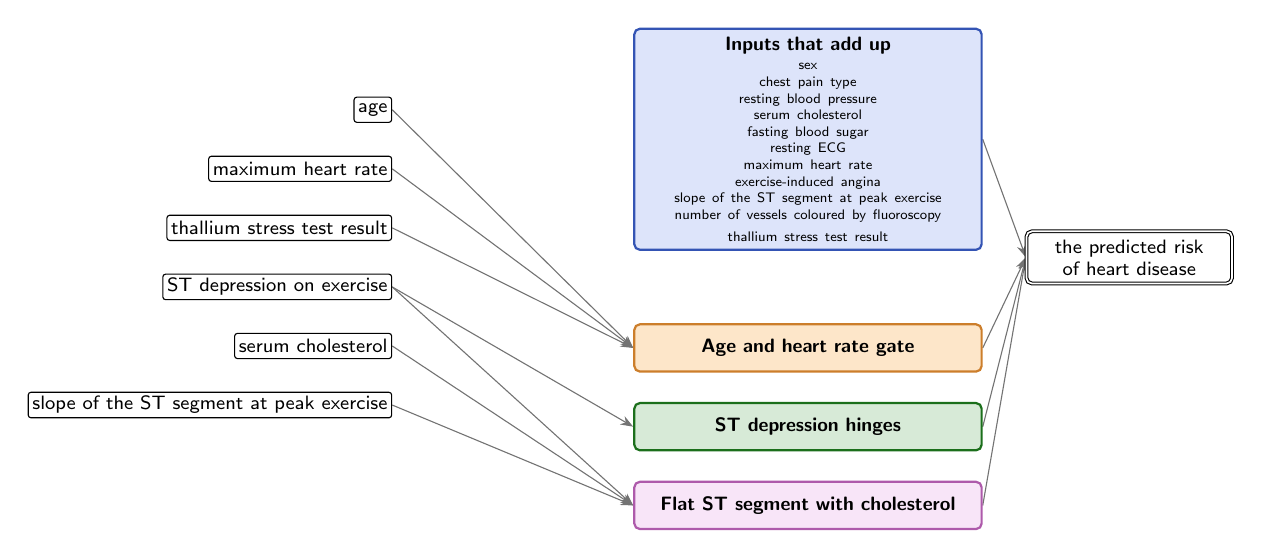
\begin{tikzpicture}[
  font=\sffamily\scriptsize, >={Stealth[length=1.6mm]},
  inp/.style={draw, rounded corners=1pt, fill=white, inner sep=1.5pt, minimum height=3.2mm, anchor=east},
  abox/.style={draw, thick, rounded corners=2pt, align=center, inner sep=3pt, minimum height=6mm, text width=42mm},
  outp/.style={draw, double, rounded corners=2pt, fill=white, align=center, inner sep=3pt, text width=24mm},
  agg/.style={draw=black!55},
]
\node[inp] (i0) at (0,1.875) {age};
\node[inp] (i1) at (0,1.125) {maximum heart rate};
\node[inp] (i2) at (0,0.375) {thallium stress test result};
\node[inp] (i3) at (0,-0.375) {ST depression on exercise};
\node[inp] (i4) at (0,-1.125) {serum cholesterol};
\node[inp] (i5) at (0,-1.875) {slope of the ST segment at peak exercise};
\node[abox, fill=RoyalBlue!18, draw=RoyalBlue!80!black] (b0) at (5.28,1.5) {\textbf{Inputs that add up}\\[1pt]{\tiny sex\\ chest pain type\\ resting blood pressure\\ serum cholesterol\\ fasting blood sugar\\ resting ECG\\ maximum heart rate\\ exercise-induced angina\\ slope of the ST segment at peak exercise\\ number of vessels coloured by fluoroscopy\\ thallium stress test result}};
\node[abox, fill=BurntOrange!18, draw=BurntOrange!80!black] (b1) at (5.28,-1.15) {\textbf{Age and heart rate gate}};
\node[abox, fill=ForestGreen!18, draw=ForestGreen!80!black] (b2) at (5.28,-2.15) {\textbf{ST depression hinges}};
\node[abox, fill=Orchid!18, draw=Orchid!80!black] (b3) at (5.28,-3.15) {\textbf{Flat ST segment with cholesterol}};
\node[outp] (out) at (9.36,0) {the predicted risk of heart disease};
\begin{scope}[on background layer]
\draw[->, agg] (b0.east) -- (out.west);
\draw[->, agg, thin] (i0.east) -- (b1.west);
\draw[->, agg, thin] (i1.east) -- (b1.west);
\draw[->, agg, thin] (i2.east) -- (b1.west);
\draw[->, agg] (b1.east) -- (out.west);
\draw[->, agg, thin] (i3.east) -- (b2.west);
\draw[->, agg] (b2.east) -- (out.west);
\draw[->, agg, thin] (i4.east) -- (b3.west);
\draw[->, agg, thin] (i3.east) -- (b3.west);
\draw[->, agg, thin] (i5.east) -- (b3.west);
\draw[->, agg] (b3.east) -- (out.west);
\end{scope}
\end{tikzpicture}}}%
\caption{The model at the level of the summary: one box per part.}
\label{fig:hearts2c1:summary}
\end{figure}
\paragraph{Inputs that add up.} \par\noindent\textit{Lowering the risk.}  These add up independently, and these lower the risk: compared with no chest pain symptoms, typical angina takes a typical patient's predicted risk from about 29\% to about 3\%, non-anginal chest pain to about 5\% and atypical angina to about 14\%; being a woman lowers it to about 3\% and fasting blood sugar above 120 mg/dL to about 14\%; and through this sum alone a higher maximum heart rate lowers it steadily, from about 32\% at 118 to about 28\% at 175 beats per minute (maximum heart rate also acts through the age and heart rate gate, below).\,{\scriptsize\textcolor{NavyBlue}{[C06, C09, C17, C07, C18, C23]}} \par\noindent\textit{Raising the risk.}  Each extra vessel coloured by fluoroscopy adds about the same, from about 29\% at 0 to about 94\% at 2 vessels, flattening out near the top because the predicted risk cannot go much higher; higher resting blood pressure raises it steadily, from about 20\% at 110 mm Hg to about 44\% at 155 mm Hg, and chest pain brought on by exercise raises it to about 43\%.\,{\scriptsize\textcolor{NavyBlue}{[C01, C08, C19]}} Through this sum alone, a flat rather than upsloping ST segment raises it to about 73\%, higher cholesterol raises it steadily from about 18\% at 193 mg/dL to about 49\% at 308 mg/dL, and a reversible defect on the thallium scan raises it to about 42\%; all three also act through the parts below.\,{\scriptsize\textcolor{NavyBlue}{[C03, C04, C20]}} \par\noindent\textit{Rare results.}  Some rarer results also count (the model has little data on this, n = 2 to 17): through this sum alone a downsloping ST segment raises the risk to about 50\% and a fixed defect on the thallium scan lowers it to about 11\%, and an ST-T wave abnormality on the resting ECG raises it to about 46\%.\,{\scriptsize\textcolor{NavyBlue}{[C10, C13, C16]}}
\paragraph{Age and heart rate gate.} This part reads age, maximum heart rate and the thallium scan, and acts on 80 of 242 training patients, 9 of whom had heart disease; for the typical patient it acts on, the predicted risk is about 4\% without it and about 1\% with it.\,{\scriptsize\textcolor{NavyBlue}{[C38]}} For patients without a reversible defect on the thallium scan, it switches on when age in years minus about 0.28 $\times$ the maximum heart rate in beats per minute is below about 11.4 (for maximum heart rates from about 71 to 202 beats per minute); 80 of 242 training patients are on that side, and 11\% of them had heart disease, against 60\% of the others.\,{\scriptsize\textcolor{NavyBlue}{[C54]}} Through it, older age raises the predicted risk steadily up to about 56 years (between 45 and 61 years for different patients), then no further for most patients, but for patients with a reversible defect on the thallium scan it rises in a jump: for a typical patient from about 12\% at 42 to about 29\% at 66 years.\,{\scriptsize\textcolor{NavyBlue}{[C30, C37]}} Across the whole model, a higher maximum heart rate lowers the risk in an uneven way, more without a reversible defect on the thallium scan (from about 32\% at 118 to about 21\% at 175 beats per minute, against about 45\% to about 40\% with one).\,{\scriptsize\textcolor{NavyBlue}{[C35]}}
\paragraph{ST depression hinges.} This part reads only ST depression on exercise and acts on 121 of 242 training patients, 77 of whom had heart disease; for the typical patient it acts on, the predicted risk is about 89\% without it and about 91\% with it.\,{\scriptsize\textcolor{NavyBlue}{[C42]}} Through it, more ST depression raises the predicted risk slowly at first, then faster, adding risk only once it rises above about 0.8 mm: for a typical patient from about 29\% at 0 mm to about 48\% at 2.8 mm.\,{\scriptsize\textcolor{NavyBlue}{[C40, C41]}}
\paragraph{Flat ST segment with cholesterol.} This part reads the slope of the ST segment, ST depression on exercise and cholesterol, and acts on 117 of 242 training patients, 78 of whom had heart disease; for the typical patient it acts on, the predicted risk is about 86\% without it and about 90\% with it.\,{\scriptsize\textcolor{NavyBlue}{[C52]}} For patients whose ST segment is not flat, it switches on when ST depression on exercise is above about 2.23 mm (for cholesterol from about 126 to 186 mg/dL), or when ST depression minus about 0.012 $\times$ the cholesterol in mg/dL is above about 0.011 (for cholesterol from about 186 to 417 mg/dL); 117 of 242 training patients are on, and 67\% of them had heart disease, against 23\% of the others.\,{\scriptsize\textcolor{NavyBlue}{[C55]}} Across the whole model, more ST depression raises the risk slowly at first, then faster, and even more so with a flat ST segment: from about 75\% to about 91\% then, against about 29\% to about 48\% otherwise.\,{\scriptsize\textcolor{NavyBlue}{[C48]}} Higher cholesterol raises it steadily across the whole model, from about 67\% to about 88\% with a flat ST segment and from about 18\% to about 49\% otherwise, while through this part it lowers the risk in an uneven way, for the typical patient the part acts on from about 91\% to about 88\%.\,{\scriptsize\textcolor{NavyBlue}{[C47, C46]}}
\paragraph{The whole network.} Figure~\ref{fig:hearts2c1:overview} (next page, landscape) draws every unit and connection of the explained model, nested by part: shaded clusters are the parts of the model and darker boxes the parts inside them; circles are hidden units (h1, h2, \ldots); each cluster's rectangle is its output, and a dashed `sum' stands for an addition the next unit does (drawn, not a unit of the model); the hexagon is the model's output. An input used by several parts is drawn under each of them (same label, dotted outline, the first copy marked with the number of copies): it is the same input, repeated for readability. Not used by the model (input columns with no connection): non-anginal pain, sugar 120 or less, normal ECG, LVH on ECG, no exercise pain, downsloping ST, normal thallium, thallium code 4.
\begin{landscape}
\begin{figure}[p]\centering
\resizebox{\linewidth}{!}{%
\definecolor{netup}{HTML}{D95F02}\definecolor{netdown}{HTML}{1B9E77}\definecolor{netmixed}{HTML}{7F7F7F}%
\begin{tikzpicture}[
  font=\sffamily\scriptsize, >={Stealth[length=1.4mm]},
  inp/.style={draw, circle, fill=white, minimum size=3.2mm, inner sep=0pt},
  hid/.style={draw, circle, fill=white, minimum size=5.2mm, inner sep=0.5pt, font=\sffamily\tiny},
  exitbox/.style={draw, thick, rectangle, fill=white, align=center, text width=17mm, minimum height=5mm, inner sep=1.5pt, font=\sffamily\tiny},
  sumbox/.style={draw, thick, dashed, rectangle, fill=white, align=center, text width=17mm, minimum height=5mm, inner sep=1.5pt, font=\sffamily\tiny},
  outp/.style={draw, thick, regular polygon, regular polygon sides=6, fill=white, minimum size=10mm, inner sep=0pt, font=\sffamily\tiny, align=center},
  stub/.style={draw, dashed, rounded corners=2pt, fill=white, align=center, inner sep=2pt, font=\sffamily\tiny, text width=15mm},
  inlab/.style={font=\sffamily\tiny, align=center, text width=15mm, inner sep=1pt, fill=white, fill opacity=0.8, text opacity=1},
  wpos/.style={draw=NavyBlue}, wneg/.style={draw=BrickRed}, wagg/.style={draw=black!45, line width=1.2pt},
  wmix/.style={draw=Plum},
]
\node[outp] (n0) at (15.81,6.15) {heart disease};
\node[exitbox] (n1476) at (28.92,3.25) {Flat ST segment with cholesterol $\uparrow$};
\node[exitbox] (n1718) at (15.94,3.25) {Age and heart rate gate $\downarrow$};
\node[hid] (n1946) at (22.18,1.9) {h3};
\node[hid] (n3195) at (15.94,1.9) {h4};
\node[hid] (n3284) at (22.18,3.25) {h5};
\node[hid] (n3464) at (28.92,1.9) {h6};
\node[sumbox] (ncsumxxannx33) at (22.18,4.6) {sum: ST depression hinges $\uparrow$};
\node[sumbox] (nxxsumxx) at (5.85,1.9) {sum: Inputs that add up};
\node[inp, draw=netdown, very thick] (ninxxsexx0xxadditive) at (3.6,-1.05) {};
\path (ninxxsexx0xxadditive.south) node[inlab, anchor=north] (labninxxsexx0xxadditive) {female $\downarrow$};
\node[inp, draw=netup, very thick] (ninxxsexx1xxadditive) at (5.4,-1.05) {};
\path (ninxxsexx1xxadditive.south) node[inlab, anchor=north] (labninxxsexx1xxadditive) {male $\uparrow$};
\node[inp, draw=netdown, very thick] (ninxxcpx1xxadditive) at (9.0,-1.05) {};
\path (ninxxcpx1xxadditive.south) node[inlab, anchor=north] (labninxxcpx1xxadditive) {typical angina $\downarrow$};
\node[inp, draw=netdown, very thick] (ninxxcpx2xxadditive) at (0.9,-2.1) {};
\path (ninxxcpx2xxadditive.south) node[inlab, anchor=north] (labninxxcpx2xxadditive) {atypical angina $\downarrow$};
\node[inp, draw=netup, very thick] (ninxxcpx4xxadditive) at (6.3,-2.1) {};
\path (ninxxcpx4xxadditive.south) node[inlab, anchor=north] (labninxxcpx4xxadditive) {no chest pain $\uparrow$};
\node[inp, draw=netup, very thick] (ninxxtrestbpsxxadditive) at (1.8,-1.05) {};
\path (ninxxtrestbpsxxadditive.south) node[inlab, anchor=north] (labninxxtrestbpsxxadditive) {blood pressure $\uparrow$};
\node[inp, draw=netdown, very thick] (ninxxfbsx1xxadditive) at (8.1,0.0) {};
\path (ninxxfbsx1xxadditive.south) node[inlab, anchor=north] (labninxxfbsx1xxadditive) {sugar above 120 $\downarrow$};
\node[inp, draw=netup, very thick] (ninxxrestecgx1xxadditive) at (0.9,0.0) {};
\path (ninxxrestecgx1xxadditive.south) node[inlab, anchor=north] (labninxxrestecgx1xxadditive) {ST-T abnormal ECG $\uparrow$};
\node[inp, draw=netup, very thick] (ninxxexangx1xxadditive) at (2.7,-2.1) {};
\path (ninxxexangx1xxadditive.south) node[inlab, anchor=north] (labninxxexangx1xxadditive) {exercise pain $\uparrow$};
\node[inp, draw=netdown, very thick] (ninxxslopex1xxadditive) at (9.9,0.0) {};
\path (ninxxslopex1xxadditive.south) node[inlab, anchor=north] (labninxxslopex1xxadditive) {upsloping ST $\downarrow$};
\node[inp, draw=netup, very thick] (ninxxcaxxadditive) at (10.8,-1.05) {};
\path (ninxxcaxxadditive.south) node[inlab, anchor=north] (labninxxcaxxadditive) {vessels $\uparrow$};
\node[inp, draw=netdown, very thick] (ninxxthalx6xxadditive) at (4.5,0.0) {};
\path (ninxxthalx6xxadditive.south) node[inlab, anchor=north] (labninxxthalx6xxadditive) {fixed defect $\downarrow$};
\node[inp, draw=netup, very thick] (ninxxagexxannx31) at (14.14,0.0) {};
\path (ninxxagexxannx31.south) node[inlab, anchor=north] (labninxxagexxannx31) {age $\uparrow$};
\node[inp, densely dotted, thick, draw=netup, very thick] (ninxxthalx7xxadditive) at (7.2,-1.05) {};
\path (ninxxthalx7xxadditive.south) node[inlab, anchor=north] (labninxxthalx7xxadditive) {reversible defect ($\times$2) $\uparrow$};
\node[inp, densely dotted, thick, draw=netup, very thick] (ninxxthalx7xxannx31) at (17.74,0.0) {};
\path (ninxxthalx7xxannx31.south) node[inlab, anchor=north] (labninxxthalx7xxannx31) {reversible defect $\uparrow$};
\node[inp, densely dotted, thick, draw=netdown, very thick] (ninxxthalachxxadditive) at (6.3,0.0) {};
\path (ninxxthalachxxadditive.south) node[inlab, anchor=north] (labninxxthalachxxadditive) {max heart rate ($\times$2) $\downarrow$};
\node[inp, densely dotted, thick, draw=netdown, very thick] (ninxxthalachxxannx31) at (15.94,0.0) {};
\path (ninxxthalachxxannx31.south) node[inlab, anchor=north] (labninxxthalachxxannx31) {max heart rate $\downarrow$};
\node[inp, densely dotted, thick, draw=netup, very thick] (ninxxcholxxadditive) at (2.7,0.0) {};
\path (ninxxcholxxadditive.south) node[inlab, anchor=north] (labninxxcholxxadditive) {cholesterol ($\times$2) $\uparrow$};
\node[inp, densely dotted, thick, draw=netdown, very thick] (ninxxcholxxannx32) at (28.92,0.0) {};
\path (ninxxcholxxannx32.south) node[inlab, anchor=north] (labninxxcholxxannx32) {cholesterol $\downarrow$};
\node[inp, densely dotted, thick, draw=netup, very thick] (ninxxslopex2xxadditive) at (4.5,-2.1) {};
\path (ninxxslopex2xxadditive.south) node[inlab, anchor=north] (labninxxslopex2xxadditive) {flat ST ($\times$2) $\uparrow$};
\node[inp, densely dotted, thick, draw=netup, very thick] (ninxxslopex2xxannx32) at (30.72,0.0) {};
\path (ninxxslopex2xxannx32.south) node[inlab, anchor=north] (labninxxslopex2xxannx32) {flat ST $\uparrow$};
\node[inp, densely dotted, thick, draw=netup, very thick] (ninxxoldpeakxxannx32) at (27.12,0.0) {};
\path (ninxxoldpeakxxannx32.south) node[inlab, anchor=north] (labninxxoldpeakxxannx32) {ST depression ($\times$2) $\uparrow$};
\node[inp, densely dotted, thick, draw=netup, very thick] (ninxxoldpeakxxannx33) at (22.18,0.0) {};
\path (ninxxoldpeakxxannx33.south) node[inlab, anchor=north] (labninxxoldpeakxxannx33) {ST depression $\uparrow$};
\begin{scope}[on background layer]
\node[fit=(nxxsumxx) , inner sep=8pt, rounded corners=5pt, fill=RoyalBlue!10, draw=RoyalBlue!45] (clu0) {};
\node[fit=(n1718) (n3195) , inner sep=8pt, rounded corners=5pt, fill=BurntOrange!10, draw=BurntOrange!45] (clu1) {};
\node[fit=(n1946) (n3284) (ncsumxxannx33) , inner sep=8pt, rounded corners=5pt, fill=ForestGreen!10, draw=ForestGreen!45] (clu2) {};
\node[fit=(n1476) (n3464) , inner sep=8pt, rounded corners=5pt, fill=Orchid!10, draw=Orchid!45] (clu3) {};
\draw[->, wneg, line width=0.51pt] (ninxxsexx0xxadditive) -- (nxxsumxx);
\draw[->, wpos, line width=0.41pt] (ninxxsexx1xxadditive) -- (nxxsumxx);
\draw[->, wneg, line width=0.31pt] (ninxxcpx1xxadditive) -- (nxxsumxx);
\draw[->, wpos, line width=0.39pt] (ninxxcpx2xxadditive) -- (nxxsumxx);
\draw[->, wpos, line width=0.60pt] (ninxxcpx4xxadditive) -- (nxxsumxx);
\draw[->, wpos, line width=0.41pt] (ninxxtrestbpsxxadditive) -- (nxxsumxx);
\draw[->, wneg, line width=0.36pt] (ninxxfbsx1xxadditive) -- (nxxsumxx);
\draw[->, wpos, line width=0.27pt] (ninxxrestecgx1xxadditive) -- (nxxsumxx);
\draw[->, wpos, line width=0.35pt] (ninxxexangx1xxadditive) -- (nxxsumxx);
\draw[->, wneg, line width=0.41pt] (ninxxslopex1xxadditive) -- (nxxsumxx);
\draw[->, wpos, line width=0.83pt] (ninxxcaxxadditive) -- (nxxsumxx);
\draw[->, wneg, line width=0.35pt] (ninxxthalx6xxadditive) -- (nxxsumxx);
\draw[->, wpos, line width=0.34pt] (n1476) -- (n0);
\draw[->, wneg, line width=0.46pt] (n1718) -- (n0);
\draw[->, wpos, line width=0.38pt] (n1946) -- (ncsumxxannx33);
\draw[->, wpos, line width=0.40pt] (n3284) -- (ncsumxxannx33);
\draw[->, wneg, line width=0.78pt] (ninxxagexxannx31) -- (n1718);
\draw[->, wpos, line width=0.60pt] (n1946) -- (n3284);
\draw[->, wneg, line width=0.51pt] (n3195) -- (n1718);
\draw[->, wneg, line width=0.38pt] (n3464) -- (n1476);
\draw[->, wpos, line width=0.35pt] (ninxxthalx7xxadditive) -- (nxxsumxx);
\draw[->, wneg, line width=0.52pt] (ninxxthalx7xxannx31) -- (n1718);
\draw[->, wpos, line width=0.63pt] (ninxxthalx7xxannx31) -- (n3195);
\draw[->, wneg, line width=0.28pt] (ninxxthalachxxadditive) -- (nxxsumxx);
\draw[->, wpos, line width=0.61pt] (ninxxthalachxxannx31) -- (n1718);
\draw[->, wpos, line width=0.46pt] (ninxxcholxxadditive) -- (nxxsumxx);
\draw[->, wpos, line width=0.60pt] (ninxxcholxxannx32) -- (n3464);
\draw[->, wpos, line width=0.42pt] (ninxxslopex2xxadditive) -- (nxxsumxx);
\draw[->, wpos, line width=0.65pt] (ninxxslopex2xxannx32) -- (n1476);
\draw[->, wpos, line width=0.52pt] (ninxxoldpeakxxannx32) -- (n1476);
\draw[->, wpos, line width=0.51pt] (ninxxoldpeakxxannx33) -- (n1946);
\draw[->, wagg] (ncsumxxannx33) -- (n0);
\draw[->, wagg] (nxxsumxx) -- (n0);
\end{scope}
\node[font=\sffamily\scriptsize\bfseries, text=RoyalBlue!55!black, anchor=south west, inner sep=1pt, fill=white, fill opacity=0.85, text opacity=1] at (clu0.north west) {Inputs that add up};
\node[font=\sffamily\scriptsize\bfseries, text=BurntOrange!55!black, anchor=south west, inner sep=1pt, fill=white, fill opacity=0.85, text opacity=1] at (clu1.north west) {Age and heart rate gate};
\node[font=\sffamily\scriptsize\bfseries, text=ForestGreen!55!black, anchor=south west, inner sep=1pt, fill=white, fill opacity=0.85, text opacity=1] at (clu2.north west) {ST depression hinges};
\node[font=\sffamily\scriptsize\bfseries, text=Orchid!55!black, anchor=south west, inner sep=1pt, fill=white, fill opacity=0.85, text opacity=1] at (clu3.north west) {Flat ST segment with cholesterol};
\end{tikzpicture}}%
\caption{Every unit and connection of the explained model, nested by part. Blue: positive weight (raises the score); red: negative weight (lowers it); thicker: larger weight. Orange outline and up arrow: raises the final prediction; teal and down arrow: lowers it; grey and double arrow: depends.}
\label{fig:hearts2c1:overview}
\end{figure}
\end{landscape}
\paragraph{Worth checking against what is known.} Worth checking: going from 0 to 2 vessels coloured moves a typical patient's predicted risk from about 29\% to about 94\%.\,{\scriptsize\textcolor{NavyBlue}{[C01]}} Worth checking: patients with typical angina get the lowest predicted risk of all chest pain types, below patients with no chest pain symptoms.\,{\scriptsize\textcolor{NavyBlue}{[C06, C09, C17]}} Worth checking: the model treats fasting blood sugar above 120 mg/dL as lowering the risk of heart disease (for a typical patient from about 29\% to about 14\%).\,{\scriptsize\textcolor{NavyBlue}{[C18]}} Worth checking: the model treats a fixed defect on the thallium scan as lowering the risk (for a typical patient from about 29\% to about 11\%), from only 15 training patients.\,{\scriptsize\textcolor{NavyBlue}{[C14]}} Worth checking: across the whole model, older age raises the predicted risk only for patients without a reversible defect on the thallium scan, and through one part only up to about 56 years.\,{\scriptsize\textcolor{NavyBlue}{[C33, C37]}}
\subsection{The model, read from the top down}
\noindent{\small Each part of the explanation in turn, from the whole model down to the smallest parts: what it does for the prediction (hypothesis), what was checked (evidence), a diagram one level down, and where to read on. The technical record of each part is in ``Technical detail'' at the end.\par}
\subsubsection{The whole model}\label{rd:ann34}
\noindent{\small Figure~\ref{fig:hearts2c1:parts-ann34} shows what feeds this part; Figure~\ref{fig:hearts2c1:units-ann34} its units and every connection into them (dashed boxes: connections from or to other parts, drawn in their own sections).\par}
\begin{figure}[H]\centering
\resizebox{!}{\ifdim\height>0.5\textheight 0.5\textheight\else\height\fi}{%
\resizebox{\ifdim\width>\linewidth\linewidth\else\width\fi}{!}{%
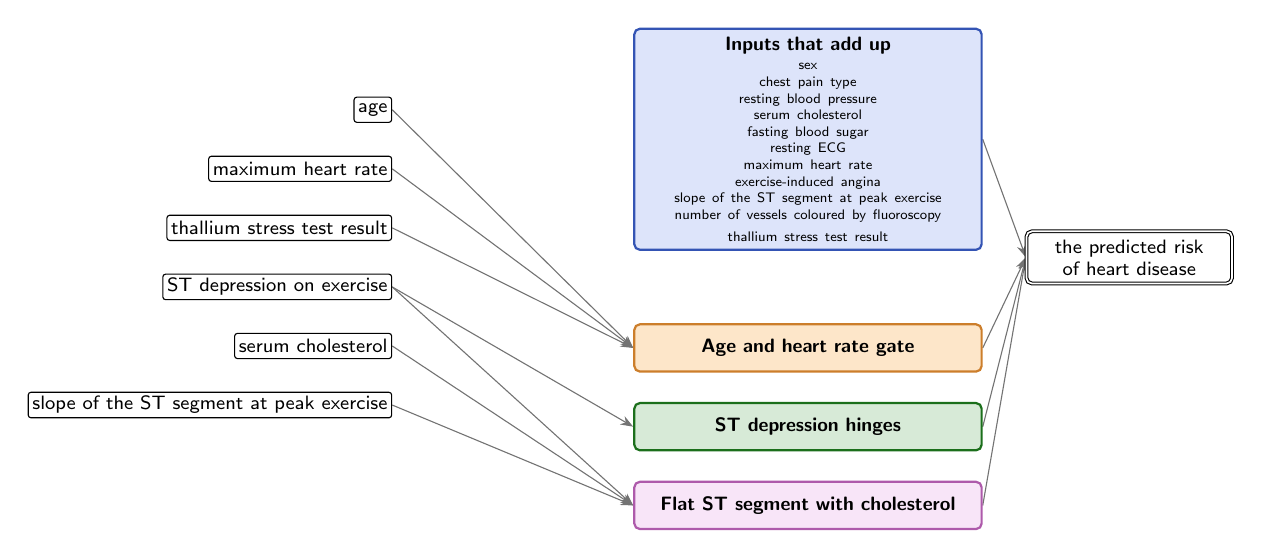
\begin{tikzpicture}[
  font=\sffamily\scriptsize, >={Stealth[length=1.6mm]},
  inp/.style={draw, rounded corners=1pt, fill=white, inner sep=1.5pt, minimum height=3.2mm, anchor=east},
  abox/.style={draw, thick, rounded corners=2pt, align=center, inner sep=3pt, minimum height=6mm, text width=42mm},
  outp/.style={draw, double, rounded corners=2pt, fill=white, align=center, inner sep=3pt, text width=24mm},
  agg/.style={draw=black!55},
]
\node[inp] (i0) at (0,1.875) {age};
\node[inp] (i1) at (0,1.125) {maximum heart rate};
\node[inp] (i2) at (0,0.375) {thallium stress test result};
\node[inp] (i3) at (0,-0.375) {ST depression on exercise};
\node[inp] (i4) at (0,-1.125) {serum cholesterol};
\node[inp] (i5) at (0,-1.875) {slope of the ST segment at peak exercise};
\node[abox, fill=RoyalBlue!18, draw=RoyalBlue!80!black] (b0) at (5.28,1.5) {\textbf{Inputs that add up}\\[1pt]{\tiny sex\\ chest pain type\\ resting blood pressure\\ serum cholesterol\\ fasting blood sugar\\ resting ECG\\ maximum heart rate\\ exercise-induced angina\\ slope of the ST segment at peak exercise\\ number of vessels coloured by fluoroscopy\\ thallium stress test result}};
\node[abox, fill=BurntOrange!18, draw=BurntOrange!80!black] (b1) at (5.28,-1.15) {\textbf{Age and heart rate gate}};
\node[abox, fill=ForestGreen!18, draw=ForestGreen!80!black] (b2) at (5.28,-2.15) {\textbf{ST depression hinges}};
\node[abox, fill=Orchid!18, draw=Orchid!80!black] (b3) at (5.28,-3.15) {\textbf{Flat ST segment with cholesterol}};
\node[outp] (out) at (9.36,0) {the predicted risk of heart disease};
\begin{scope}[on background layer]
\draw[->, agg] (b0.east) -- (out.west);
\draw[->, agg, thin] (i0.east) -- (b1.west);
\draw[->, agg, thin] (i1.east) -- (b1.west);
\draw[->, agg, thin] (i2.east) -- (b1.west);
\draw[->, agg] (b1.east) -- (out.west);
\draw[->, agg, thin] (i3.east) -- (b2.west);
\draw[->, agg] (b2.east) -- (out.west);
\draw[->, agg, thin] (i4.east) -- (b3.west);
\draw[->, agg, thin] (i3.east) -- (b3.west);
\draw[->, agg, thin] (i5.east) -- (b3.west);
\draw[->, agg] (b3.east) -- (out.west);
\end{scope}
\end{tikzpicture}}}%
\caption{The whole model: what feeds it, one level down.}
\label{fig:hearts2c1:parts-ann34}
\end{figure}
\begin{figure}[H]\centering
\resizebox{\ifdim\width>\linewidth\linewidth\else\width\fi}{!}{%
\definecolor{netup}{HTML}{D95F02}\definecolor{netdown}{HTML}{1B9E77}\definecolor{netmixed}{HTML}{7F7F7F}%
\begin{tikzpicture}[
  font=\sffamily\scriptsize, >={Stealth[length=1.4mm]},
  inp/.style={draw, circle, fill=white, minimum size=3.2mm, inner sep=0pt},
  hid/.style={draw, circle, fill=white, minimum size=5.2mm, inner sep=0.5pt, font=\sffamily\tiny},
  exitbox/.style={draw, thick, rectangle, fill=white, align=center, text width=17mm, minimum height=5mm, inner sep=1.5pt, font=\sffamily\tiny},
  sumbox/.style={draw, thick, dashed, rectangle, fill=white, align=center, text width=17mm, minimum height=5mm, inner sep=1.5pt, font=\sffamily\tiny},
  outp/.style={draw, thick, regular polygon, regular polygon sides=6, fill=white, minimum size=10mm, inner sep=0pt, font=\sffamily\tiny, align=center},
  stub/.style={draw, dashed, rounded corners=2pt, fill=white, align=center, inner sep=2pt, font=\sffamily\tiny, text width=15mm},
  inlab/.style={font=\sffamily\tiny, align=center, text width=15mm, inner sep=1pt, fill=white, fill opacity=0.8, text opacity=1},
  wpos/.style={draw=NavyBlue}, wneg/.style={draw=BrickRed}, wagg/.style={draw=black!45, line width=1.2pt},
  wmix/.style={draw=Plum},
]
\node[outp] (n0) at (9.32,3.45) {heart disease};
\node[inp, draw=netdown, very thick] (ninxxsexx0) at (3.6,-1.05) {};
\path (ninxxsexx0.south) node[inlab, anchor=north] (labninxxsexx0) {female $\downarrow$};
\node[sumbox] (nxxsumxx) at (5.85,1.9) {sum: Inputs that add up};
\node[inp, draw=netup, very thick] (ninxxsexx1) at (5.4,-1.05) {};
\path (ninxxsexx1.south) node[inlab, anchor=north] (labninxxsexx1) {male $\uparrow$};
\node[inp, draw=netdown, very thick] (ninxxcpx1) at (9.0,-1.05) {};
\path (ninxxcpx1.south) node[inlab, anchor=north] (labninxxcpx1) {typical angina $\downarrow$};
\node[inp, draw=netdown, very thick] (ninxxcpx2) at (0.9,-2.1) {};
\path (ninxxcpx2.south) node[inlab, anchor=north] (labninxxcpx2) {atypical angina $\downarrow$};
\node[inp, draw=netup, very thick] (ninxxcpx4) at (6.3,-2.1) {};
\path (ninxxcpx4.south) node[inlab, anchor=north] (labninxxcpx4) {no chest pain $\uparrow$};
\node[inp, draw=netup, very thick] (ninxxtrestbps) at (1.8,-1.05) {};
\path (ninxxtrestbps.south) node[inlab, anchor=north] (labninxxtrestbps) {blood pressure $\uparrow$};
\node[inp, draw=netdown, very thick] (ninxxfbsx1) at (8.1,0.0) {};
\path (ninxxfbsx1.south) node[inlab, anchor=north] (labninxxfbsx1) {sugar above 120 $\downarrow$};
\node[inp, draw=netup, very thick] (ninxxrestecgx1) at (0.9,0.0) {};
\path (ninxxrestecgx1.south) node[inlab, anchor=north] (labninxxrestecgx1) {ST-T abnormal ECG $\uparrow$};
\node[inp, draw=netup, very thick] (ninxxexangx1) at (2.7,-2.1) {};
\path (ninxxexangx1.south) node[inlab, anchor=north] (labninxxexangx1) {exercise pain $\uparrow$};
\node[inp, draw=netdown, very thick] (ninxxslopex1) at (9.9,0.0) {};
\path (ninxxslopex1.south) node[inlab, anchor=north] (labninxxslopex1) {upsloping ST $\downarrow$};
\node[inp, draw=netup, very thick] (ninxxca) at (10.8,-1.05) {};
\path (ninxxca.south) node[inlab, anchor=north] (labninxxca) {vessels $\uparrow$};
\node[inp, draw=netdown, very thick] (ninxxthalx6) at (4.5,0.0) {};
\path (ninxxthalx6.south) node[inlab, anchor=north] (labninxxthalx6) {fixed defect $\downarrow$};
\node[stub] (nfromxxFlatxSTxsegmentxwithxcholesterol) at (15.94,0.0) {from Flat ST segment with cholesterol};
\node[stub] (nfromxxAgexandxheartxratexgate) at (14.14,0.0) {from Age and heart rate gate};
\node[stub] (nfromxxSTxdepressionxhinges) at (17.74,0.0) {from ST depression hinges};
\node[inp, draw=netup, very thick] (ninxxthalx7) at (7.2,-1.05) {};
\path (ninxxthalx7.south) node[inlab, anchor=north] (labninxxthalx7) {reversible defect $\uparrow$};
\node[inp, draw=netdown, very thick] (ninxxthalach) at (6.3,0.0) {};
\path (ninxxthalach.south) node[inlab, anchor=north] (labninxxthalach) {max heart rate $\downarrow$};
\node[inp, draw=netup, very thick] (ninxxchol) at (2.7,0.0) {};
\path (ninxxchol.south) node[inlab, anchor=north] (labninxxchol) {cholesterol $\uparrow$};
\node[inp, draw=netup, very thick] (ninxxslopex2) at (4.5,-2.1) {};
\path (ninxxslopex2.south) node[inlab, anchor=north] (labninxxslopex2) {flat ST $\uparrow$};
\begin{scope}[on background layer]
\node[fit=(nxxsumxx) , inner sep=8pt, rounded corners=5pt, fill=RoyalBlue!10, draw=RoyalBlue!45] (clu0) {};
\draw[->, wneg, line width=0.51pt] (ninxxsexx0) -- (nxxsumxx);
\draw[->, wpos, line width=0.41pt] (ninxxsexx1) -- (nxxsumxx);
\draw[->, wneg, line width=0.31pt] (ninxxcpx1) -- (nxxsumxx);
\draw[->, wpos, line width=0.39pt] (ninxxcpx2) -- (nxxsumxx);
\draw[->, wpos, line width=0.60pt] (ninxxcpx4) -- (nxxsumxx);
\draw[->, wpos, line width=0.41pt] (ninxxtrestbps) -- (nxxsumxx);
\draw[->, wneg, line width=0.36pt] (ninxxfbsx1) -- (nxxsumxx);
\draw[->, wpos, line width=0.27pt] (ninxxrestecgx1) -- (nxxsumxx);
\draw[->, wpos, line width=0.35pt] (ninxxexangx1) -- (nxxsumxx);
\draw[->, wneg, line width=0.41pt] (ninxxslopex1) -- (nxxsumxx);
\draw[->, wpos, line width=0.83pt] (ninxxca) -- (nxxsumxx);
\draw[->, wneg, line width=0.35pt] (ninxxthalx6) -- (nxxsumxx);
\draw[->, wpos, line width=0.34pt] (nfromxxFlatxSTxsegmentxwithxcholesterol) -- (n0);
\draw[->, wneg, line width=0.46pt] (nfromxxAgexandxheartxratexgate) -- (n0);
\draw[->, wpos, line width=0.38pt] (nfromxxSTxdepressionxhinges) -- (n0);
\draw[->, wpos, line width=0.40pt] (nfromxxSTxdepressionxhinges) -- (n0);
\draw[->, wpos, line width=0.35pt] (ninxxthalx7) -- (nxxsumxx);
\draw[->, wneg, line width=0.28pt] (ninxxthalach) -- (nxxsumxx);
\draw[->, wpos, line width=0.46pt] (ninxxchol) -- (nxxsumxx);
\draw[->, wpos, line width=0.42pt] (ninxxslopex2) -- (nxxsumxx);
\draw[->, wagg] (nxxsumxx) -- (n0);
\end{scope}
\node[font=\sffamily\scriptsize\bfseries, text=RoyalBlue!55!black, anchor=south west, inner sep=1pt, fill=white, fill opacity=0.85, text opacity=1] at (clu0.north west) {Inputs that add up};
\end{tikzpicture}}%
\caption{The whole model: its units and every connection into them. Blue: positive weight (raises the score); red: negative weight (lowers it); thicker: larger weight. Orange outline and up arrow: raises the final prediction; teal and down arrow: lowers it; grey and double arrow: depends.}
\label{fig:hearts2c1:units-ann34}
\end{figure}
\paragraph{Hypothesis.} The model adds up its inputs into one score: the vessels coloured (each extra vessel adding about the same), the ST segment, chest pain type and sex each move the predicted risk on their own, and three parts add to that sum: one for age and maximum heart rate, one for ST depression and one for the ST segment with cholesterol.\,{\scriptsize\textcolor{NavyBlue}{[C29, C01, C02, C06, C07]}}
\paragraph{Evidence.} It is made up of the inputs that feed the score directly and three parts, the age and heart rate gate, the ST depression hinges and the flat ST segment with cholesterol part (each explained below); the score is their sum, which was checked on all 242 training patients.\,{\scriptsize\textcolor{NavyBlue}{[C29]}} Age and ST depression on exercise do not feed the score directly, so they act only through these parts.\,{\scriptsize\textcolor{NavyBlue}{[C29, C30, C40]}} Changing one input at a time across the whole model, a flat rather than upsloping ST segment takes a typical patient's predicted risk from about 29\% to about 77\%, against about 73\% through the sum alone.\,{\scriptsize\textcolor{NavyBlue}{[C02, C03]}} Across the whole model, a higher maximum heart rate lowers it in an uneven way, from about 32\% at 118 to about 21\% at 175 beats per minute, against about 28\% through the sum alone, where it falls steadily.\,{\scriptsize\textcolor{NavyBlue}{[C22, C23]}} Across the whole model, a fixed defect on the thallium scan lowers it to about 11\% (the model has little data on this, n = 15), and a reversible defect raises it to about 42\%.\,{\scriptsize\textcolor{NavyBlue}{[C14, C21]}}
\par\noindent{\small Evidence plots: Figure~\ref{fig:hearts2c1:plot-ann34-0}.\par}
\begin{figure}[H]\centering
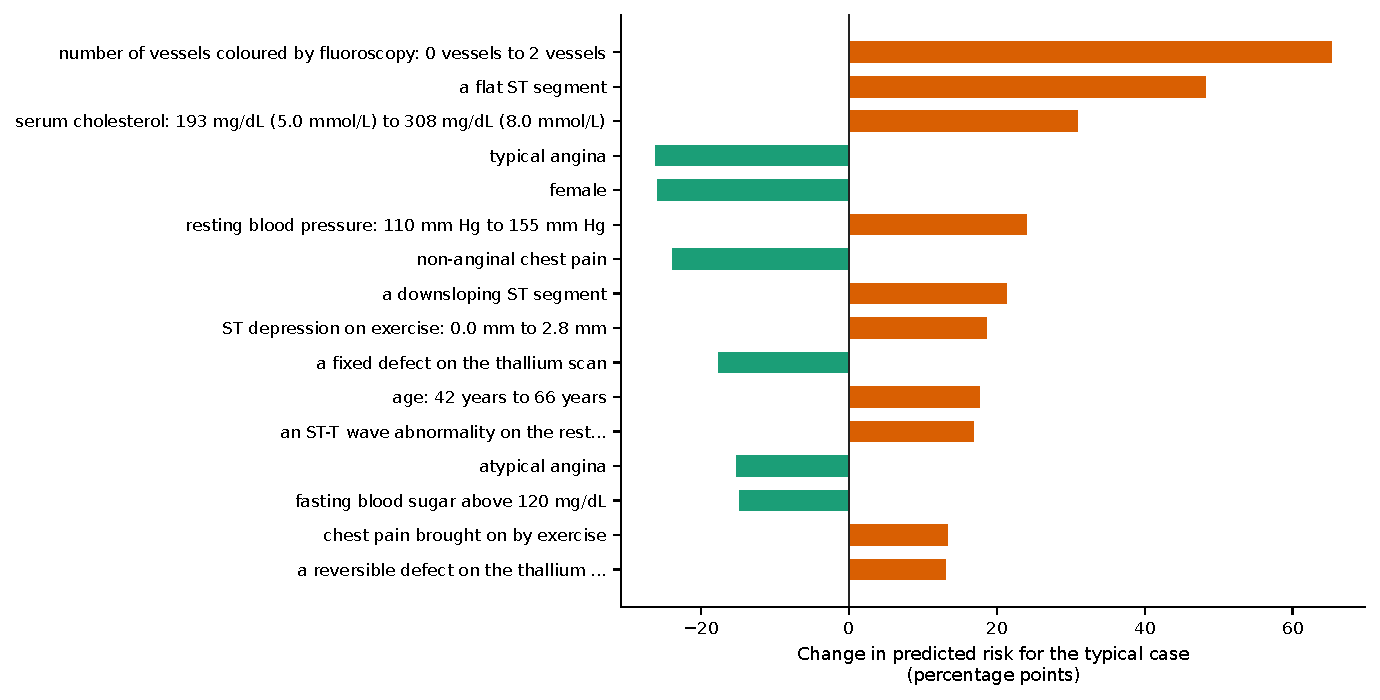
\includegraphics[width=\linewidth,height=0.88\textheight,keepaspectratio]{figures/heart-s2-c1/ann_34-effects.pdf}
\caption{The whole model: Each input's change in the predicted value for the typical case across the whole model, largest first (orange: raises it, teal: lowers it).}
\label{fig:hearts2c1:plot-ann34-0}
\end{figure}
\par\smallskip\noindent{\small \textbf{Dive deeper:} Age and heart rate gate (\ref{rd:ann31}); ST depression hinges (\ref{rd:ann33}); Flat ST segment with cholesterol (\ref{rd:ann32}). Technical detail: \ref{tech:ann34}.\par}
\subsubsection{Age and heart rate gate}\label{rd:ann31}
\noindent{\footnotesize Part of: The whole model (\ref{rd:ann34}).\par}
\noindent{\small Figure~\ref{fig:hearts2c1:parts-ann31} shows what feeds this part; Figure~\ref{fig:hearts2c1:units-ann31} its units and every connection into them (dashed boxes: connections from or to other parts, drawn in their own sections).\par}
\begin{figure}[H]\centering
\resizebox{!}{\ifdim\height>0.5\textheight 0.5\textheight\else\height\fi}{%
\resizebox{\ifdim\width>\linewidth\linewidth\else\width\fi}{!}{%
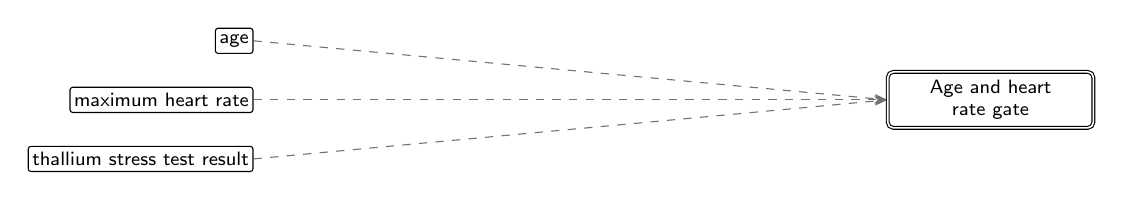
\begin{tikzpicture}[
  font=\sffamily\scriptsize, >={Stealth[length=1.6mm]},
  inp/.style={draw, rounded corners=1pt, fill=white, inner sep=1.5pt, minimum height=3.2mm, anchor=east},
  abox/.style={draw, thick, rounded corners=2pt, align=center, inner sep=3pt, minimum height=6mm, text width=42mm},
  outp/.style={draw, double, rounded corners=2pt, fill=white, align=center, inner sep=3pt, text width=24mm},
  agg/.style={draw=black!55},
]
\node[inp] (i0) at (0,0.75) {age};
\node[inp] (i1) at (0,-0.0) {maximum heart rate};
\node[inp] (i2) at (0,-0.75) {thallium stress test result};
\node[outp] (out) at (9.36,0) {Age and heart rate gate};
\begin{scope}[on background layer]
\draw[->, agg, thin, dashed] (i0.east) -- (out.west);
\draw[->, agg, thin, dashed] (i1.east) -- (out.west);
\draw[->, agg, thin, dashed] (i2.east) -- (out.west);
\end{scope}
\end{tikzpicture}}}%
\caption{Age and heart rate gate: what feeds it, one level down.}
\label{fig:hearts2c1:parts-ann31}
\end{figure}
\begin{figure}[H]\centering
\resizebox{\ifdim\width>\linewidth\linewidth\else\width\fi}{!}{%
\definecolor{netup}{HTML}{D95F02}\definecolor{netdown}{HTML}{1B9E77}\definecolor{netmixed}{HTML}{7F7F7F}%
\begin{tikzpicture}[
  font=\sffamily\scriptsize, >={Stealth[length=1.4mm]},
  inp/.style={draw, circle, fill=white, minimum size=3.2mm, inner sep=0pt},
  hid/.style={draw, circle, fill=white, minimum size=5.2mm, inner sep=0.5pt, font=\sffamily\tiny},
  exitbox/.style={draw, thick, rectangle, fill=white, align=center, text width=17mm, minimum height=5mm, inner sep=1.5pt, font=\sffamily\tiny},
  sumbox/.style={draw, thick, dashed, rectangle, fill=white, align=center, text width=17mm, minimum height=5mm, inner sep=1.5pt, font=\sffamily\tiny},
  outp/.style={draw, thick, regular polygon, regular polygon sides=6, fill=white, minimum size=10mm, inner sep=0pt, font=\sffamily\tiny, align=center},
  stub/.style={draw, dashed, rounded corners=2pt, fill=white, align=center, inner sep=2pt, font=\sffamily\tiny, text width=15mm},
  inlab/.style={font=\sffamily\tiny, align=center, text width=15mm, inner sep=1pt, fill=white, fill opacity=0.8, text opacity=1},
  wpos/.style={draw=NavyBlue}, wneg/.style={draw=BrickRed}, wagg/.style={draw=black!45, line width=1.2pt},
  wmix/.style={draw=Plum},
]
\node[exitbox] (n1718) at (2.7,3.25) {Age and heart rate gate $\downarrow$};
\node[hid] (n3195) at (2.7,1.9) {h4};
\node[inp, draw=netup, very thick] (ninxxage) at (0.9,0.0) {};
\path (ninxxage.south) node[inlab, anchor=north] (labninxxage) {age $\uparrow$};
\node[inp, draw=netup, very thick] (ninxxthalx7) at (4.5,0.0) {};
\path (ninxxthalx7.south) node[inlab, anchor=north] (labninxxthalx7) {reversible defect $\uparrow$};
\node[inp, draw=netdown, very thick] (ninxxthalach) at (2.7,0.0) {};
\path (ninxxthalach.south) node[inlab, anchor=north] (labninxxthalach) {max heart rate $\downarrow$};
\node[stub] (ntoxxthexmodelxoutput) at (2.7,4.8) {to the model output};
\begin{scope}[on background layer]
\node[fit=(n1718) (n3195) , inner sep=8pt, rounded corners=5pt, fill=BurntOrange!10, draw=BurntOrange!45] (clu0) {};
\draw[->, wneg, line width=0.78pt] (ninxxage) -- (n1718);
\draw[->, wneg, line width=0.51pt] (n3195) -- (n1718);
\draw[->, wneg, line width=0.52pt] (ninxxthalx7) -- (n1718);
\draw[->, wpos, line width=0.63pt] (ninxxthalx7) -- (n3195);
\draw[->, wpos, line width=0.61pt] (ninxxthalach) -- (n1718);
\draw[->, wneg, line width=0.46pt] (n1718) -- (ntoxxthexmodelxoutput);
\end{scope}
\node[font=\sffamily\scriptsize\bfseries, text=BurntOrange!55!black, anchor=south west, inner sep=1pt, fill=white, fill opacity=0.85, text opacity=1] at (clu0.north west) {Age and heart rate gate};
\end{tikzpicture}}%
\caption{Age and heart rate gate: its units and every connection into them. Blue: positive weight (raises the score); red: negative weight (lowers it); thicker: larger weight. Orange outline and up arrow: raises the final prediction; teal and down arrow: lowers it; grey and double arrow: depends.}
\label{fig:hearts2c1:units-ann31}
\end{figure}
\paragraph{Hypothesis.} This part lowers the predicted risk for patients whose age is low relative to their maximum heart rate; for the typical patient it acts on, a reversible defect on the thallium scan raises the risk through it from about 1\% to about 4\%.\,{\scriptsize\textcolor{NavyBlue}{[C54, C32]}}
\paragraph{Evidence.} For patients without a reversible defect on the thallium scan, it switches on when age in years minus about 0.28 $\times$ the maximum heart rate in beats per minute is below about 11.4 (for maximum heart rates from about 71 to 202 beats per minute); 80 of 242 training patients are on that side, and 11\% of them had heart disease, against 60\% of the others.\,{\scriptsize\textcolor{NavyBlue}{[C54]}} Through it, older age raises the predicted risk steadily up to about 56 years (between 45 and 61 years for different patients), then no further for most patients, but for patients with a reversible defect on the thallium scan it rises in a jump: for a typical patient from about 12\% at 42 to about 29\% at 66 years.\,{\scriptsize\textcolor{NavyBlue}{[C30, C37]}} Across the whole model, older age raises the risk, then no further, only if the thallium scan shows no reversible defect: from about 12\% to about 29\%, while with one it stays at about 42\%.\,{\scriptsize\textcolor{NavyBlue}{[C33]}} A higher maximum heart rate lowers the risk through it in an uneven way, from about 29\% at 118 to about 22\% at 175 beats per minute, and across the whole model it lowers it more without a reversible defect (from about 32\% to about 21\%, against about 45\% to about 40\%).\,{\scriptsize\textcolor{NavyBlue}{[C31, C35]}} Its formula reproduces the part exactly on all 242 training patients.\,{\scriptsize\textcolor{NavyBlue}{[C39]}}
\par\noindent{\small Evidence plots: Figure~\ref{fig:hearts2c1:plot-ann31-0}, Figure~\ref{fig:hearts2c1:plot-ann31-1}, Figure~\ref{fig:hearts2c1:plot-ann31-2}, Figure~\ref{fig:hearts2c1:plot-ann31-3}, Figure~\ref{fig:hearts2c1:plot-ann31-4}, Figure~\ref{fig:hearts2c1:plot-ann31-5}, Figure~\ref{fig:hearts2c1:plot-ann31-6}, Figure~\ref{fig:hearts2c1:plot-ann31-7}.\par}
\par\medskip\noindent\textbf{Worked example: reading this part.} Figure~\ref{fig:hearts2c1:plot-ann31-3} maps the part's own output over its main inputs. In the grey region it is switched off and adds nothing; past the black line it switches on, and the colour shows how much it adds to the score. The line is the rule in the claim (C54): it switches on when age minus about 0.28 $\times$ maximum heart rate below about 11.4 (for maximum heart rate from about 71.0 to 202). 80 of 242 training patients lie on the 'on' side, and 11\% of them had heart disease, against 60\% of the others: the 'on' side holds mostly hollow points, so the part picks out low-risk cases. Figure~\ref{fig:hearts2c1:plot-ann31-4} cuts the map into slices: the hinge moves as the other input changes, which is what a tilted line means. Figure~\ref{fig:hearts2c1:plot-ann31-5} shows what this does to the final prediction for the typical case.\par
\par\noindent{\small Figure~\ref{fig:hearts2c1:plot-ann31-6} shows this part's own output, unit h2: over its two main inputs, with the line where it switches on.\par}
\begin{figure}[H]\centering
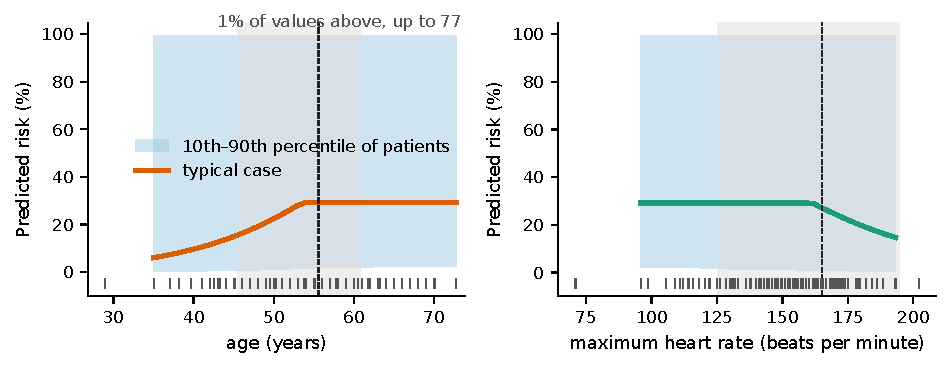
\includegraphics[width=\linewidth,height=0.88\textheight,keepaspectratio]{figures/heart-s2-c1/ann_31-response.pdf}
\caption{Age and heart rate gate: Response curves through this part: the typical case (bold), the 10th to 90th percentile of individual patients (band), the fold or step point (dashed) with its spread across them (grey), and the observed values (ticks).}
\label{fig:hearts2c1:plot-ann31-0}
\end{figure}
\begin{figure}[H]\centering
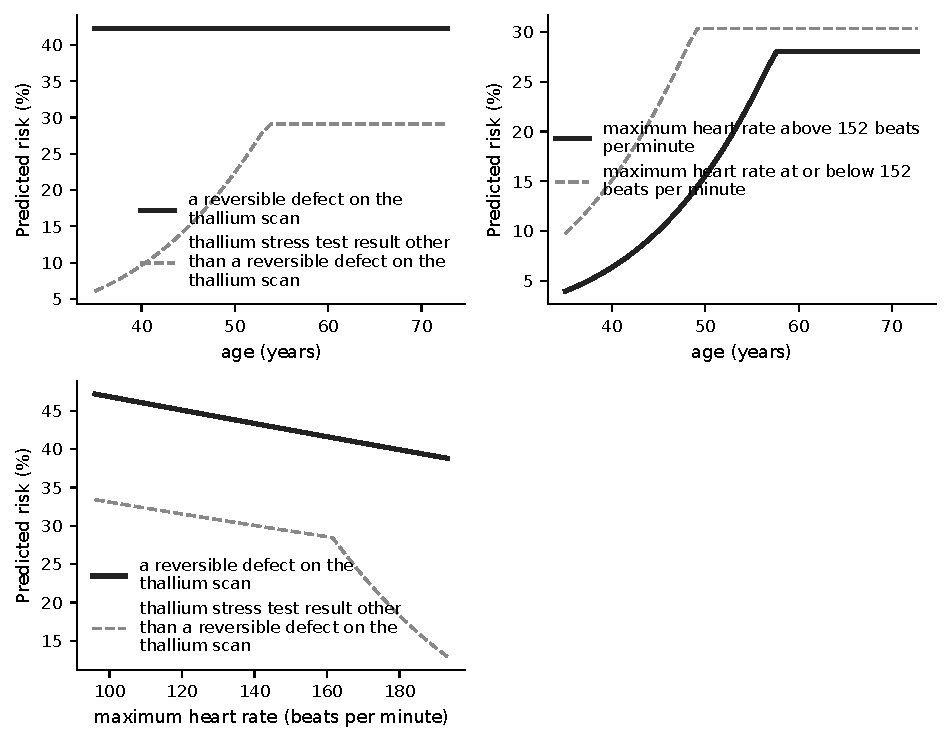
\includegraphics[width=\linewidth,height=0.88\textheight,keepaspectratio]{figures/heart-s2-c1/ann_31-interaction.pdf}
\caption{Age and heart rate gate: How the effect differs between groups: one curve per group, for the typical case of each group.}
\label{fig:hearts2c1:plot-ann31-1}
\end{figure}
\begin{figure}[H]\centering
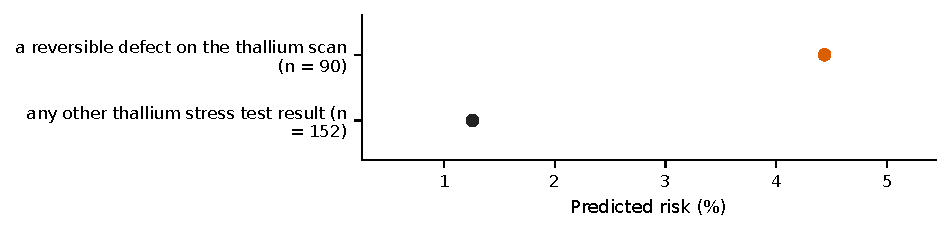
\includegraphics[width=\linewidth,height=0.88\textheight,keepaspectratio]{figures/heart-s2-c1/ann_31-categories-small.pdf}
\caption{Age and heart rate gate: The predicted value for the typical case at each level, through this part (n = training patients; grey: fewer than 20).}
\label{fig:hearts2c1:plot-ann31-2}
\end{figure}
\begin{figure}[H]\centering
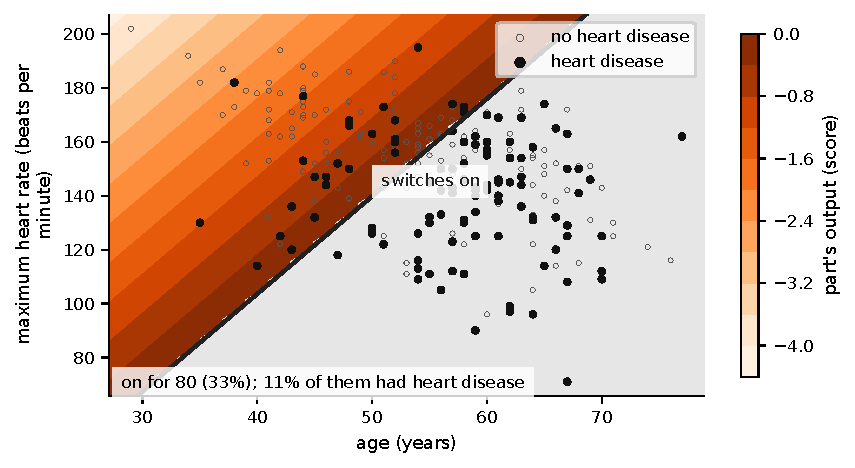
\includegraphics[width=\linewidth,height=0.88\textheight,keepaspectratio]{figures/heart-s2-c1/ann_31-deep-map.pdf}
\caption{Age and heart rate gate: The part's own output over its two numeric inputs, other inputs at the typical case: colour where it is on, flat grey where it is switched off, the black line where it switches on; training patients as hollow (no event) and filled (event) points, so the part can be seen catching the events (the predicted-chance overlay was harder to read).}
\label{fig:hearts2c1:plot-ann31-3}
\end{figure}
\begin{figure}[H]\centering
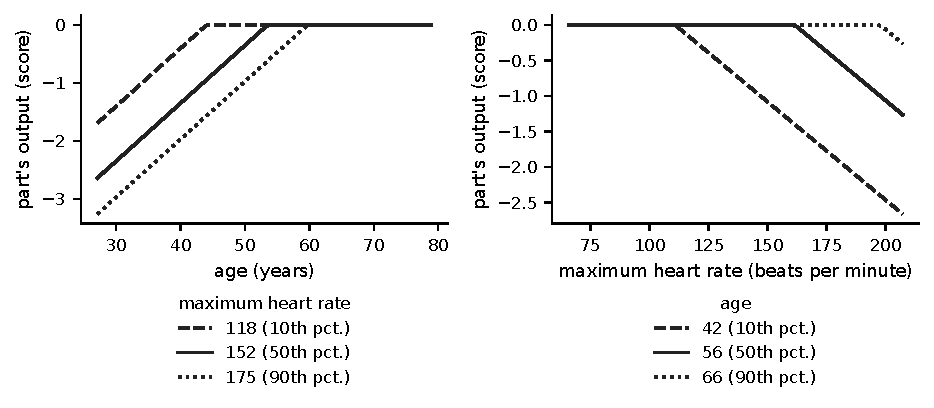
\includegraphics[width=\linewidth,height=0.88\textheight,keepaspectratio]{figures/heart-s2-c1/ann_31-deep-slices.pdf}
\caption{Age and heart rate gate: Slices of the same map: the part's own output against each input at three values of the other, so the tilted boundary shows as a shifting hinge.}
\label{fig:hearts2c1:plot-ann31-4}
\end{figure}
\begin{figure}[H]\centering
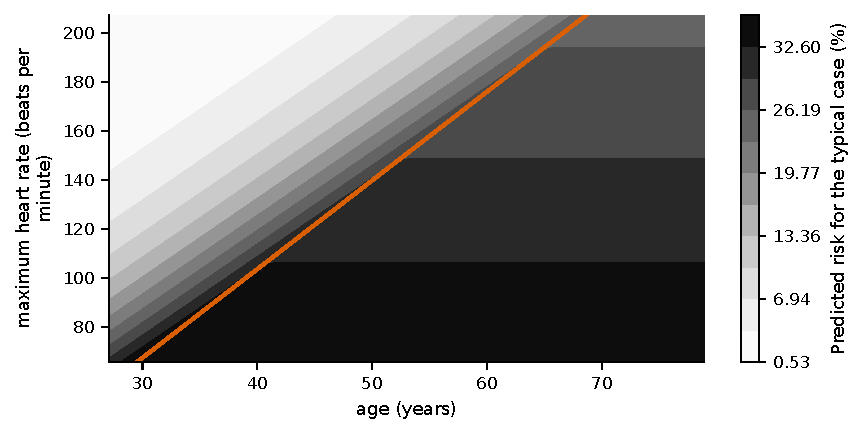
\includegraphics[width=\linewidth,height=0.88\textheight,keepaspectratio]{figures/heart-s2-c1/ann_31-deep-risk.pdf}
\caption{Age and heart rate gate: The same map on the final scale: the predicted value for the typical case, with the switch-on line (orange).}
\label{fig:hearts2c1:plot-ann31-5}
\end{figure}
\begin{figure}[H]\centering
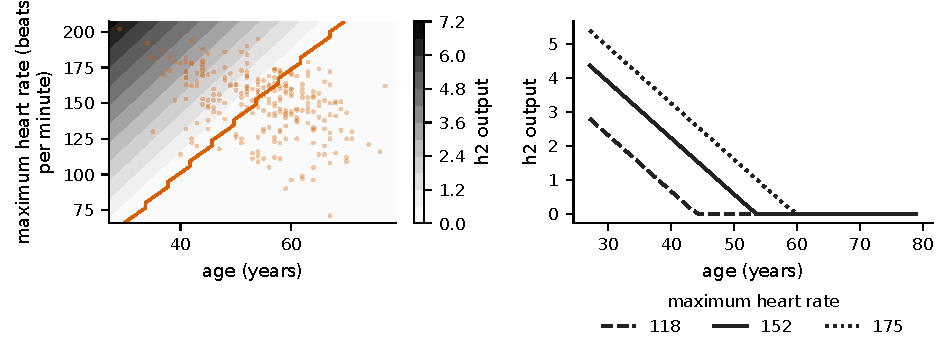
\includegraphics[width=\linewidth,height=0.88\textheight,keepaspectratio]{figures/heart-s2-c1/ann_31-partial-1718.pdf}
\caption{Age and heart rate gate: This part's own output, unit h2 (the output of 'Age and heart rate gate'), on its own scale (its activation), with every other input at the typical case; it is active for 80 of 242. Left: its output over its two main inputs (orange line: where it switches on; dots: the data); right: slices at three values of the second input.}
\label{fig:hearts2c1:plot-ann31-6}
\end{figure}
\begin{figure}[H]\centering
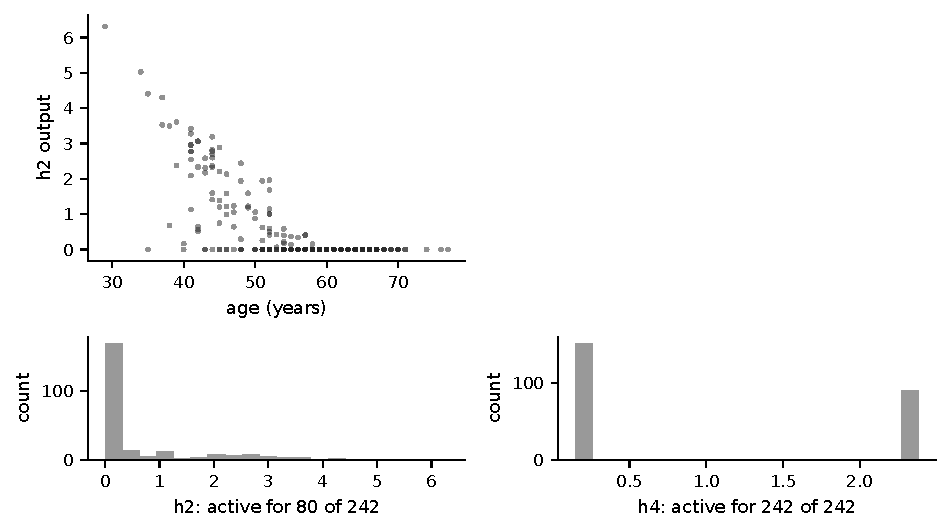
\includegraphics[width=\linewidth,height=0.88\textheight,keepaspectratio]{figures/heart-s2-c1/ann_31-units.pdf}
\caption{Age and heart rate gate: This part's hidden units: each unit's output against its main numeric input (top) and how often it is active (bottom).}
\label{fig:hearts2c1:plot-ann31-7}
\end{figure}
\par\smallskip\noindent{\small Technical detail: \ref{tech:ann31}.\par}
\subsubsection{ST depression hinges}\label{rd:ann33}
\noindent{\footnotesize Part of: The whole model (\ref{rd:ann34}).\par}
\noindent{\small Figure~\ref{fig:hearts2c1:parts-ann33} shows what feeds this part; Figure~\ref{fig:hearts2c1:units-ann33} its units and every connection into them (dashed boxes: connections from or to other parts, drawn in their own sections).\par}
\begin{figure}[H]\centering
\resizebox{!}{\ifdim\height>0.5\textheight 0.5\textheight\else\height\fi}{%
\resizebox{\ifdim\width>\linewidth\linewidth\else\width\fi}{!}{%
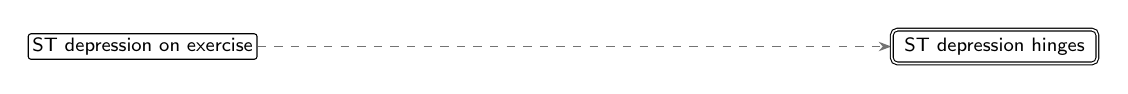
\begin{tikzpicture}[
  font=\sffamily\scriptsize, >={Stealth[length=1.6mm]},
  inp/.style={draw, rounded corners=1pt, fill=white, inner sep=1.5pt, minimum height=3.2mm, anchor=east},
  abox/.style={draw, thick, rounded corners=2pt, align=center, inner sep=3pt, minimum height=6mm, text width=42mm},
  outp/.style={draw, double, rounded corners=2pt, fill=white, align=center, inner sep=3pt, text width=24mm},
  agg/.style={draw=black!55},
]
\node[inp] (i0) at (0,-0.0) {ST depression on exercise};
\node[outp] (out) at (9.36,0) {ST depression hinges};
\begin{scope}[on background layer]
\draw[->, agg, thin, dashed] (i0.east) -- (out.west);
\end{scope}
\end{tikzpicture}}}%
\caption{ST depression hinges: what feeds it, one level down.}
\label{fig:hearts2c1:parts-ann33}
\end{figure}
\begin{figure}[H]\centering
\resizebox{\ifdim\width>\linewidth\linewidth\else\width\fi}{!}{%
\definecolor{netup}{HTML}{D95F02}\definecolor{netdown}{HTML}{1B9E77}\definecolor{netmixed}{HTML}{7F7F7F}%
\begin{tikzpicture}[
  font=\sffamily\scriptsize, >={Stealth[length=1.4mm]},
  inp/.style={draw, circle, fill=white, minimum size=3.2mm, inner sep=0pt},
  hid/.style={draw, circle, fill=white, minimum size=5.2mm, inner sep=0.5pt, font=\sffamily\tiny},
  exitbox/.style={draw, thick, rectangle, fill=white, align=center, text width=17mm, minimum height=5mm, inner sep=1.5pt, font=\sffamily\tiny},
  sumbox/.style={draw, thick, dashed, rectangle, fill=white, align=center, text width=17mm, minimum height=5mm, inner sep=1.5pt, font=\sffamily\tiny},
  outp/.style={draw, thick, regular polygon, regular polygon sides=6, fill=white, minimum size=10mm, inner sep=0pt, font=\sffamily\tiny, align=center},
  stub/.style={draw, dashed, rounded corners=2pt, fill=white, align=center, inner sep=2pt, font=\sffamily\tiny, text width=15mm},
  inlab/.style={font=\sffamily\tiny, align=center, text width=15mm, inner sep=1pt, fill=white, fill opacity=0.8, text opacity=1},
  wpos/.style={draw=NavyBlue}, wneg/.style={draw=BrickRed}, wagg/.style={draw=black!45, line width=1.2pt},
  wmix/.style={draw=Plum},
]
\node[hid] (n1946) at (2.0,1.9) {h3};
\node[hid] (n3284) at (2.0,3.25) {h5};
\node[inp, draw=netup, very thick] (ninxxoldpeak) at (2.0,0.0) {};
\path (ninxxoldpeak.south) node[inlab, anchor=north] (labninxxoldpeak) {ST depression $\uparrow$};
\node[stub] (ntoxxthexmodelxoutput) at (2.0,4.8) {to the model output};
\begin{scope}[on background layer]
\node[fit=(n1946) (n3284) , inner sep=8pt, rounded corners=5pt, fill=ForestGreen!10, draw=ForestGreen!45] (clu0) {};
\draw[->, wpos, line width=0.60pt] (n1946) -- (n3284);
\draw[->, wpos, line width=0.51pt] (ninxxoldpeak) -- (n1946);
\draw[->, wpos, line width=0.38pt] (n1946) -- (ntoxxthexmodelxoutput);
\draw[->, wpos, line width=0.40pt] (n3284) -- (ntoxxthexmodelxoutput);
\end{scope}
\node[font=\sffamily\scriptsize\bfseries, text=ForestGreen!55!black, anchor=south west, inner sep=1pt, fill=white, fill opacity=0.85, text opacity=1] at (clu0.north west) {ST depression hinges};
\end{tikzpicture}}%
\caption{ST depression hinges: its units and every connection into them. Blue: positive weight (raises the score); red: negative weight (lowers it); thicker: larger weight. Orange outline and up arrow: raises the final prediction; teal and down arrow: lowers it; grey and double arrow: depends.}
\label{fig:hearts2c1:units-ann33}
\end{figure}
\paragraph{Hypothesis.} This part raises the predicted risk with ST depression on exercise, slowly at first, then faster, adding risk only once it rises above about 0.8 mm.\,{\scriptsize\textcolor{NavyBlue}{[C40, C41]}}
\paragraph{Evidence.} It acts on 121 of 242 training patients, 77 of whom had heart disease; for the typical patient it acts on, the predicted risk is about 89\% without it and about 91\% with it.\,{\scriptsize\textcolor{NavyBlue}{[C42]}} Through it, more ST depression raises the risk slowly at first, then faster, adding risk only once it rises above about 0.8 mm: for a typical patient from about 29\% at 0 mm to about 48\% at 2.8 mm.\,{\scriptsize\textcolor{NavyBlue}{[C40, C41]}} Its formula reproduces the part exactly on all 242 training patients.\,{\scriptsize\textcolor{NavyBlue}{[C43]}}
\par\noindent{\small Evidence plots: Figure~\ref{fig:hearts2c1:plot-ann33-0}, Figure~\ref{fig:hearts2c1:plot-ann33-1}, Figure~\ref{fig:hearts2c1:plot-ann33-2}, Figure~\ref{fig:hearts2c1:plot-ann33-3}.\par}
\par\noindent{\small Figure~\ref{fig:hearts2c1:plot-ann33-1} shows this part's own output, unit h3: it switches on at about 0.7582 mm of ST depression on exercise, and is zero below.\par}
\par\noindent{\small Figure~\ref{fig:hearts2c1:plot-ann33-2} shows this part's own output, unit h5: it switches on at about 1.666 mm of ST depression on exercise, and is zero below.\par}
\begin{figure}[H]\centering
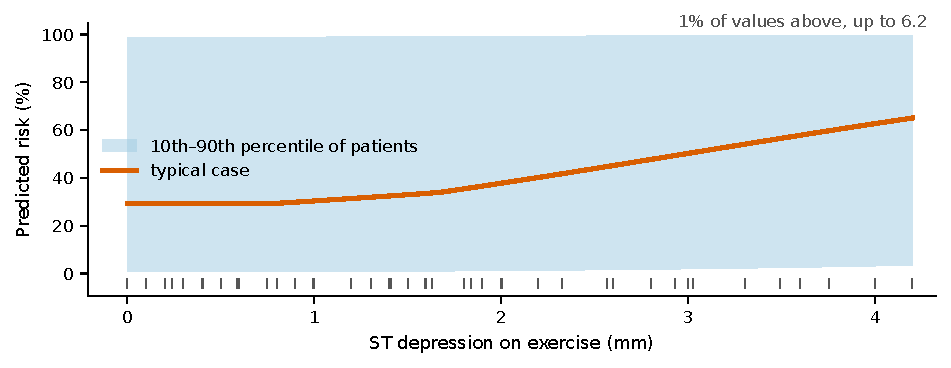
\includegraphics[width=\linewidth,height=0.88\textheight,keepaspectratio]{figures/heart-s2-c1/ann_33-response.pdf}
\caption{ST depression hinges: Response curves through this part: the typical case (bold), the 10th to 90th percentile of individual patients (band), the fold or step point (dashed) with its spread across them (grey), and the observed values (ticks).}
\label{fig:hearts2c1:plot-ann33-0}
\end{figure}
\begin{figure}[H]\centering
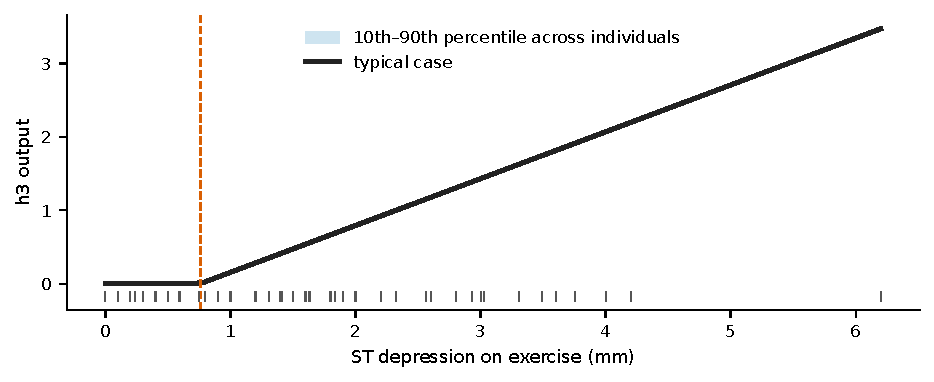
\includegraphics[width=\linewidth,height=0.88\textheight,keepaspectratio]{figures/heart-s2-c1/ann_33-partial-1946.pdf}
\caption{ST depression hinges: This part's own output, unit h3 (the output of 'ST depression hinges'), on its own scale (its activation), with every other input at the typical case; it is active for 121 of 242. Bold: the typical case; band: 10th to 90th percentile across individuals; dashed: where it switches on; ticks: the data.}
\label{fig:hearts2c1:plot-ann33-1}
\end{figure}
\begin{figure}[H]\centering
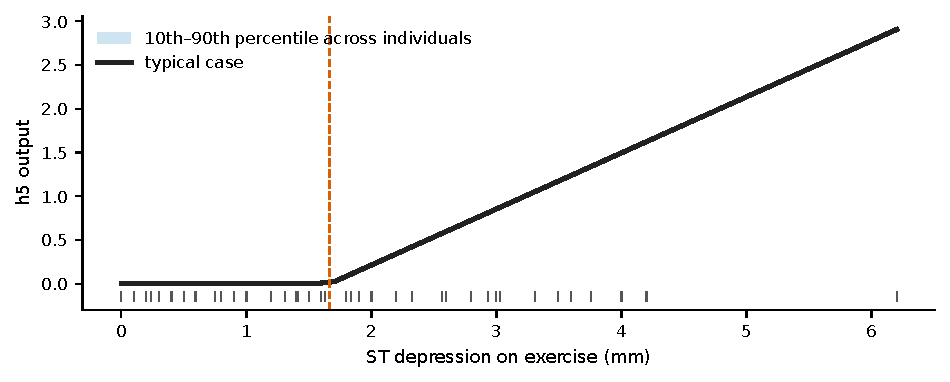
\includegraphics[width=\linewidth,height=0.88\textheight,keepaspectratio]{figures/heart-s2-c1/ann_33-partial-3284.pdf}
\caption{ST depression hinges: This part's own output, unit h5 (the output of 'ST depression hinges'), on its own scale (its activation), with every other input at the typical case; it is active for 58 of 242. Bold: the typical case; band: 10th to 90th percentile across individuals; dashed: where it switches on; ticks: the data.}
\label{fig:hearts2c1:plot-ann33-2}
\end{figure}
\begin{figure}[H]\centering
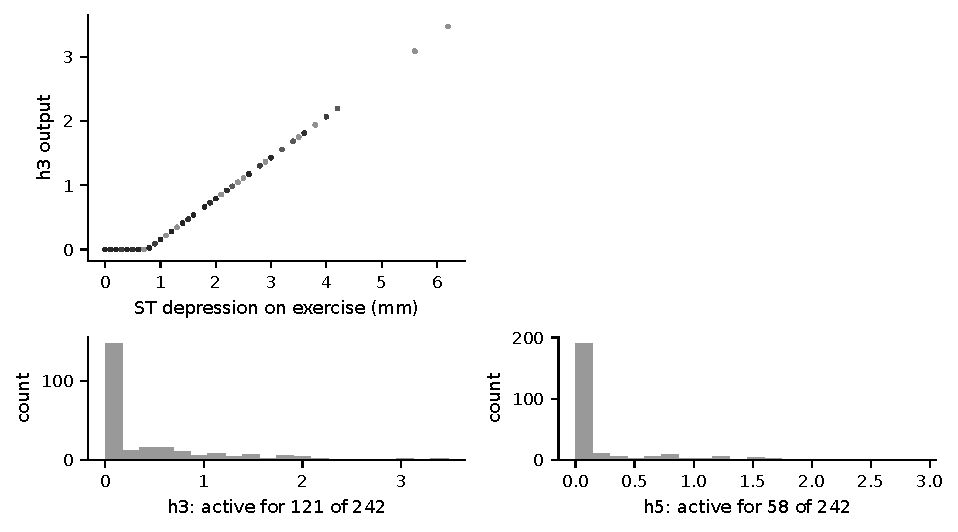
\includegraphics[width=\linewidth,height=0.88\textheight,keepaspectratio]{figures/heart-s2-c1/ann_33-units.pdf}
\caption{ST depression hinges: This part's hidden units: each unit's output against its main numeric input (top) and how often it is active (bottom).}
\label{fig:hearts2c1:plot-ann33-3}
\end{figure}
\par\smallskip\noindent{\small Technical detail: \ref{tech:ann33}.\par}
\subsubsection{Flat ST segment with cholesterol}\label{rd:ann32}
\noindent{\footnotesize Part of: The whole model (\ref{rd:ann34}).\par}
\noindent{\small Figure~\ref{fig:hearts2c1:parts-ann32} shows what feeds this part; Figure~\ref{fig:hearts2c1:units-ann32} its units and every connection into them (dashed boxes: connections from or to other parts, drawn in their own sections).\par}
\begin{figure}[H]\centering
\resizebox{!}{\ifdim\height>0.5\textheight 0.5\textheight\else\height\fi}{%
\resizebox{\ifdim\width>\linewidth\linewidth\else\width\fi}{!}{%
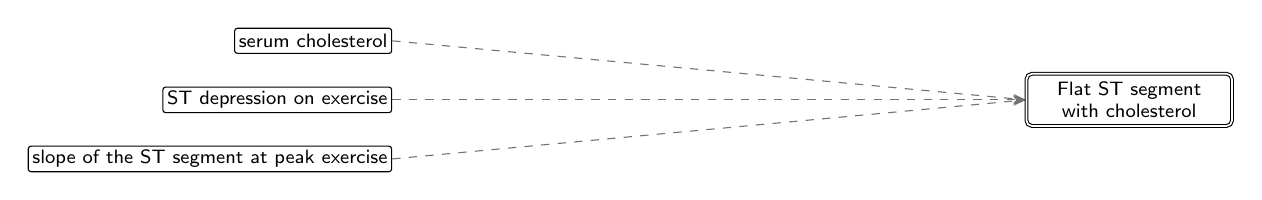
\begin{tikzpicture}[
  font=\sffamily\scriptsize, >={Stealth[length=1.6mm]},
  inp/.style={draw, rounded corners=1pt, fill=white, inner sep=1.5pt, minimum height=3.2mm, anchor=east},
  abox/.style={draw, thick, rounded corners=2pt, align=center, inner sep=3pt, minimum height=6mm, text width=42mm},
  outp/.style={draw, double, rounded corners=2pt, fill=white, align=center, inner sep=3pt, text width=24mm},
  agg/.style={draw=black!55},
]
\node[inp] (i0) at (0,0.75) {serum cholesterol};
\node[inp] (i1) at (0,-0.0) {ST depression on exercise};
\node[inp] (i2) at (0,-0.75) {slope of the ST segment at peak exercise};
\node[outp] (out) at (9.36,0) {Flat ST segment with cholesterol};
\begin{scope}[on background layer]
\draw[->, agg, thin, dashed] (i0.east) -- (out.west);
\draw[->, agg, thin, dashed] (i1.east) -- (out.west);
\draw[->, agg, thin, dashed] (i2.east) -- (out.west);
\end{scope}
\end{tikzpicture}}}%
\caption{Flat ST segment with cholesterol: what feeds it, one level down.}
\label{fig:hearts2c1:parts-ann32}
\end{figure}
\begin{figure}[H]\centering
\resizebox{\ifdim\width>\linewidth\linewidth\else\width\fi}{!}{%
\definecolor{netup}{HTML}{D95F02}\definecolor{netdown}{HTML}{1B9E77}\definecolor{netmixed}{HTML}{7F7F7F}%
\begin{tikzpicture}[
  font=\sffamily\scriptsize, >={Stealth[length=1.4mm]},
  inp/.style={draw, circle, fill=white, minimum size=3.2mm, inner sep=0pt},
  hid/.style={draw, circle, fill=white, minimum size=5.2mm, inner sep=0.5pt, font=\sffamily\tiny},
  exitbox/.style={draw, thick, rectangle, fill=white, align=center, text width=17mm, minimum height=5mm, inner sep=1.5pt, font=\sffamily\tiny},
  sumbox/.style={draw, thick, dashed, rectangle, fill=white, align=center, text width=17mm, minimum height=5mm, inner sep=1.5pt, font=\sffamily\tiny},
  outp/.style={draw, thick, regular polygon, regular polygon sides=6, fill=white, minimum size=10mm, inner sep=0pt, font=\sffamily\tiny, align=center},
  stub/.style={draw, dashed, rounded corners=2pt, fill=white, align=center, inner sep=2pt, font=\sffamily\tiny, text width=15mm},
  inlab/.style={font=\sffamily\tiny, align=center, text width=15mm, inner sep=1pt, fill=white, fill opacity=0.8, text opacity=1},
  wpos/.style={draw=NavyBlue}, wneg/.style={draw=BrickRed}, wagg/.style={draw=black!45, line width=1.2pt},
  wmix/.style={draw=Plum},
]
\node[hid] (n3464) at (3.2,1.9) {h6};
\node[exitbox] (n1476) at (3.2,3.25) {Flat ST segment with cholesterol $\uparrow$};
\node[inp, draw=netdown, very thick] (ninxxchol) at (3.2,0.0) {};
\path (ninxxchol.south) node[inlab, anchor=north] (labninxxchol) {cholesterol $\downarrow$};
\node[inp, draw=netup, very thick] (ninxxslopex2) at (5.0,0.0) {};
\path (ninxxslopex2.south) node[inlab, anchor=north] (labninxxslopex2) {flat ST $\uparrow$};
\node[inp, draw=netup, very thick] (ninxxoldpeak) at (1.4,0.0) {};
\path (ninxxoldpeak.south) node[inlab, anchor=north] (labninxxoldpeak) {ST depression $\uparrow$};
\node[stub] (ntoxxthexmodelxoutput) at (3.2,4.8) {to the model output};
\begin{scope}[on background layer]
\node[fit=(n3464) (n1476) , inner sep=8pt, rounded corners=5pt, fill=Orchid!10, draw=Orchid!45] (clu0) {};
\draw[->, wneg, line width=0.38pt] (n3464) -- (n1476);
\draw[->, wpos, line width=0.60pt] (ninxxchol) -- (n3464);
\draw[->, wpos, line width=0.65pt] (ninxxslopex2) -- (n1476);
\draw[->, wpos, line width=0.52pt] (ninxxoldpeak) -- (n1476);
\draw[->, wpos, line width=0.34pt] (n1476) -- (ntoxxthexmodelxoutput);
\end{scope}
\node[font=\sffamily\scriptsize\bfseries, text=Orchid!55!black, anchor=south west, inner sep=1pt, fill=white, fill opacity=0.85, text opacity=1] at (clu0.north west) {Flat ST segment with cholesterol};
\end{tikzpicture}}%
\caption{Flat ST segment with cholesterol: its units and every connection into them. Blue: positive weight (raises the score); red: negative weight (lowers it); thicker: larger weight. Orange outline and up arrow: raises the final prediction; teal and down arrow: lowers it; grey and double arrow: depends.}
\label{fig:hearts2c1:units-ann32}
\end{figure}
\paragraph{Hypothesis.} This part raises the predicted risk mainly for patients with a flat ST segment, and makes ST depression on exercise count more for them, rising slowly at first, then faster.\,{\scriptsize\textcolor{NavyBlue}{[C44, C48]}}
\paragraph{Evidence.} It acts on 117 of 242 training patients, 78 of whom had heart disease; for the typical patient it acts on, the predicted risk is about 86\% without it and about 90\% with it.\,{\scriptsize\textcolor{NavyBlue}{[C52]}} For patients whose ST segment is not flat, it switches on when ST depression on exercise is above about 2.23 mm (for cholesterol from about 126 to 186 mg/dL), or when ST depression minus about 0.012 $\times$ the cholesterol in mg/dL is above about 0.011 (for cholesterol from about 186 to 417 mg/dL); 117 of 242 training patients are on, and 67\% of them had heart disease, against 23\% of the others.\,{\scriptsize\textcolor{NavyBlue}{[C55]}} Through it, a flat ST segment raises a typical patient's predicted risk from about 29\% to about 34\%; for the typical patient it acts on, more ST depression raises it in an uneven way from about 87\% to about 92\%, and higher cholesterol lowers it in an uneven way from about 91\% to about 88\%.\,{\scriptsize\textcolor{NavyBlue}{[C44, C45, C46]}} Across the whole model, more ST depression raises the risk slowly at first, then faster, from about 75\% to about 91\% with a flat ST segment, against about 29\% to about 48\% otherwise.\,{\scriptsize\textcolor{NavyBlue}{[C48]}} Its formula reproduces the part exactly on all 242 training patients.\,{\scriptsize\textcolor{NavyBlue}{[C53]}}
\par\noindent{\small Evidence plots: Figure~\ref{fig:hearts2c1:plot-ann32-0}, Figure~\ref{fig:hearts2c1:plot-ann32-1}, Figure~\ref{fig:hearts2c1:plot-ann32-2}, Figure~\ref{fig:hearts2c1:plot-ann32-3}, Figure~\ref{fig:hearts2c1:plot-ann32-4}, Figure~\ref{fig:hearts2c1:plot-ann32-5}, Figure~\ref{fig:hearts2c1:plot-ann32-6}, Figure~\ref{fig:hearts2c1:plot-ann32-7}.\par}
\par\medskip\noindent\textbf{Worked example: reading this part.} Figure~\ref{fig:hearts2c1:plot-ann32-3} maps the part's own output over its main inputs. In the grey region it is switched off and adds nothing; past the black line it switches on, and the colour shows how much it adds to the score. The line is the rule in the claim (C55): it switches on when ST depression on exercise above about 2.23 (for serum cholesterol from about 126 to 186); ST depression on exercise minus about 0.012 $\times$ serum cholesterol above about 0.011 (for serum cholesterol from about 186 to 417). 117 of 242 training patients lie on the 'on' side, and 67\% of them had heart disease, against 23\% of the others: the filled points crowd on the 'on' side. Figure~\ref{fig:hearts2c1:plot-ann32-4} cuts the map into slices: the hinge moves as the other input changes, which is what a tilted line means. Figure~\ref{fig:hearts2c1:plot-ann32-5} shows what this does to the final prediction for the typical case.\par
\par\noindent{\small Figure~\ref{fig:hearts2c1:plot-ann32-6} shows this part's own output, unit h1: it switches on at about 2.935 mm of ST depression on exercise, and is zero below.\par}
\begin{figure}[H]\centering
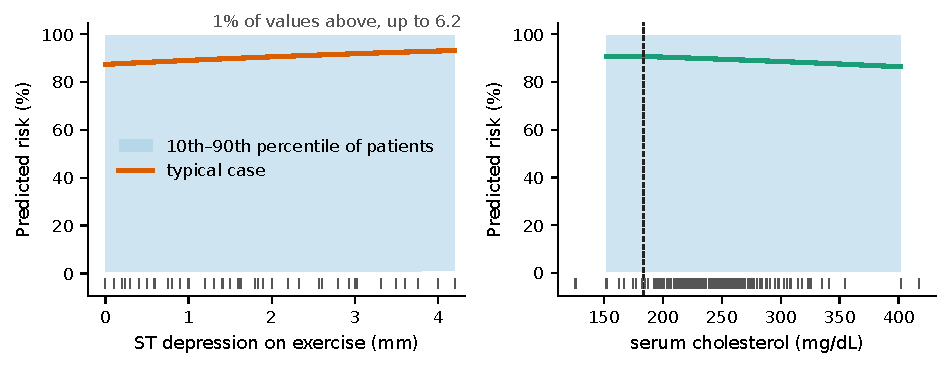
\includegraphics[width=\linewidth,height=0.88\textheight,keepaspectratio]{figures/heart-s2-c1/ann_32-response.pdf}
\caption{Flat ST segment with cholesterol: Response curves through this part: the typical case (bold), the 10th to 90th percentile of individual patients (band), the fold or step point (dashed) with its spread across them (grey), and the observed values (ticks).}
\label{fig:hearts2c1:plot-ann32-0}
\end{figure}
\begin{figure}[H]\centering
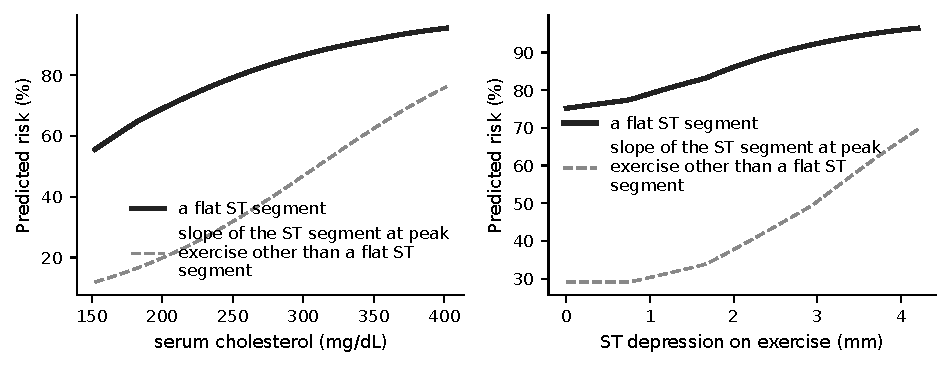
\includegraphics[width=\linewidth,height=0.88\textheight,keepaspectratio]{figures/heart-s2-c1/ann_32-interaction.pdf}
\caption{Flat ST segment with cholesterol: How the effect differs between groups: one curve per group, for the typical case of each group.}
\label{fig:hearts2c1:plot-ann32-1}
\end{figure}
\begin{figure}[H]\centering
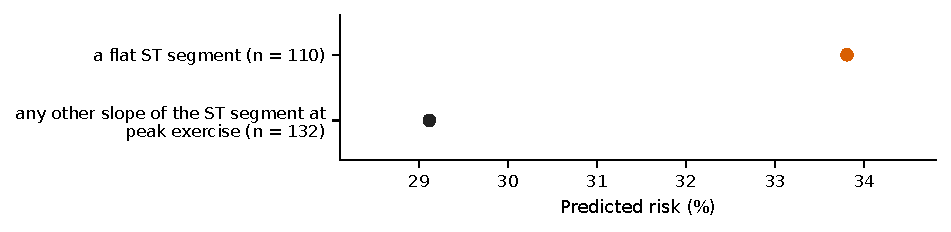
\includegraphics[width=\linewidth,height=0.88\textheight,keepaspectratio]{figures/heart-s2-c1/ann_32-categories-small.pdf}
\caption{Flat ST segment with cholesterol: The predicted value for the typical case at each level, through this part (n = training patients; grey: fewer than 20).}
\label{fig:hearts2c1:plot-ann32-2}
\end{figure}
\begin{figure}[H]\centering
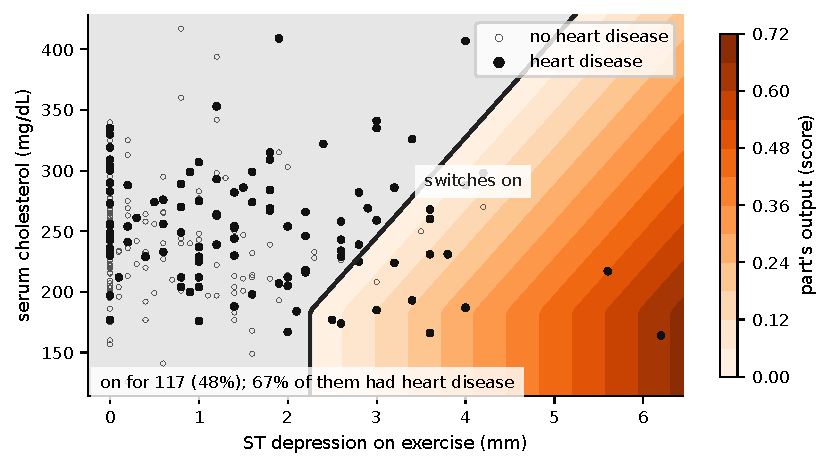
\includegraphics[width=\linewidth,height=0.88\textheight,keepaspectratio]{figures/heart-s2-c1/ann_32-deep-map.pdf}
\caption{Flat ST segment with cholesterol: The part's own output over its two numeric inputs, other inputs at the typical case: colour where it is on, flat grey where it is switched off, the black line where it switches on; training patients as hollow (no event) and filled (event) points, so the part can be seen catching the events (the predicted-chance overlay was harder to read).}
\label{fig:hearts2c1:plot-ann32-3}
\end{figure}
\begin{figure}[H]\centering
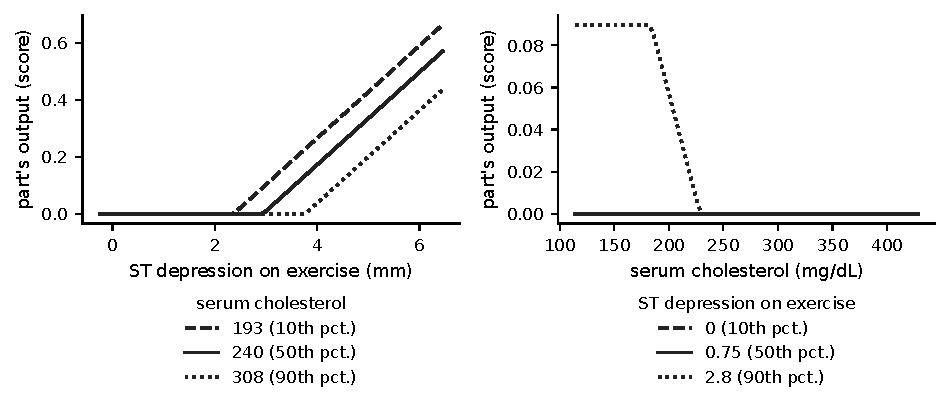
\includegraphics[width=\linewidth,height=0.88\textheight,keepaspectratio]{figures/heart-s2-c1/ann_32-deep-slices.pdf}
\caption{Flat ST segment with cholesterol: Slices of the same map: the part's own output against each input at three values of the other, so the tilted boundary shows as a shifting hinge.}
\label{fig:hearts2c1:plot-ann32-4}
\end{figure}
\begin{figure}[H]\centering
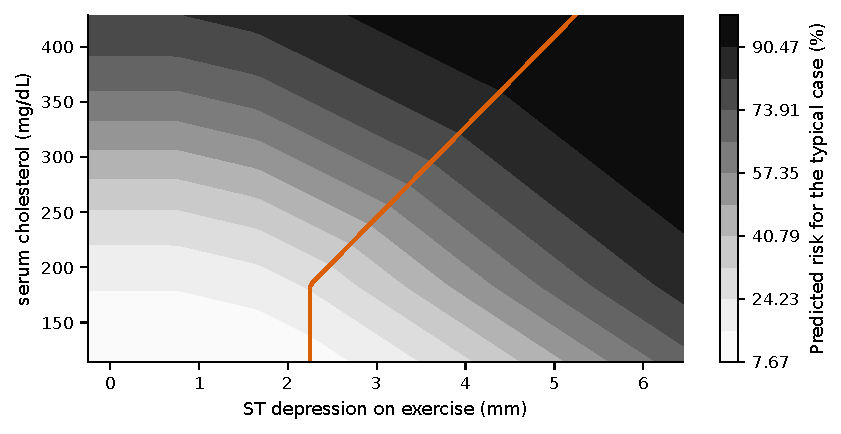
\includegraphics[width=\linewidth,height=0.88\textheight,keepaspectratio]{figures/heart-s2-c1/ann_32-deep-risk.pdf}
\caption{Flat ST segment with cholesterol: The same map on the final scale: the predicted value for the typical case, with the switch-on line (orange).}
\label{fig:hearts2c1:plot-ann32-5}
\end{figure}
\begin{figure}[H]\centering
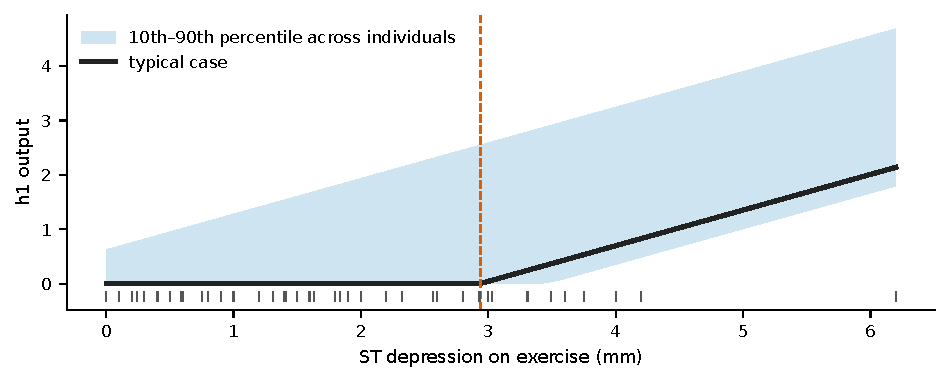
\includegraphics[width=\linewidth,height=0.88\textheight,keepaspectratio]{figures/heart-s2-c1/ann_32-partial-1476.pdf}
\caption{Flat ST segment with cholesterol: This part's own output, unit h1 (the output of 'Flat ST segment with cholesterol'), on its own scale (its activation), with every other input at the typical case; it is active for 117 of 242. Bold: the typical case; band: 10th to 90th percentile across individuals; dashed: where it switches on; ticks: the data.}
\label{fig:hearts2c1:plot-ann32-6}
\end{figure}
\begin{figure}[H]\centering
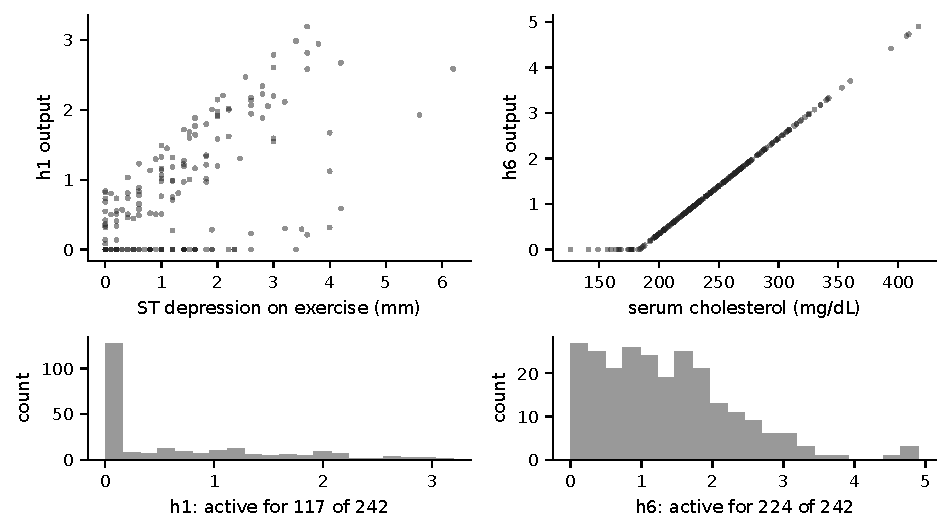
\includegraphics[width=\linewidth,height=0.88\textheight,keepaspectratio]{figures/heart-s2-c1/ann_32-units.pdf}
\caption{Flat ST segment with cholesterol: This part's hidden units: each unit's output against its main numeric input (top) and how often it is active (bottom).}
\label{fig:hearts2c1:plot-ann32-7}
\end{figure}
\par\smallskip\noindent{\small Technical detail: \ref{tech:ann32}.\par}
\subsection{Not supported by the model}
\begin{itemize}\setlength\itemsep{0pt}\small
\item C49: interaction claim about serum cholesterol and ST depression during exercise (compared with rest) in part ann\_\allowbreak{}32: not supported by the model (the group difference is below 0.1 log-odds).
\end{itemize}
\clearpage\section*{Technical detail: heart-s2-c1}
\addcontentsline{toc}{section}{Technical detail: heart-s2-c1}
\noindent{\small The record behind each part: the original hypothesis, the closed form, and every claim with its estimate (log-odds and odds ratio), range across patients, n and test check.\par}
\renewcommand{\thesubsection}{T.\arabic{subsection}}\setcounter{subsection}{0}
\subsection{The whole model}\label{tech:ann34}
\noindent{\footnotesize Annotation ann\_\allowbreak{}34 (heart\_\allowbreak{}disease\_\allowbreak{}logit). Reads: age, sex, chest pain type, resting blood pressure, serum cholesterol, fasting blood sugar, resting ECG, maximum heart rate reached during the exercise test, exercise-induced angina, ST depression during exercise (compared with rest), slope of the ST segment at peak exercise, number of major vessels coloured by fluoroscopy, thallium stress test result.\par}
\paragraph{Original hypothesis (unchanged).} Root: p = sigmoid(z), z = -0.227 + LINEAR CORE - 0.605*\allowbreak{}age\_\allowbreak{}hr\_\allowbreak{}reserve\_\allowbreak{}gate + 0.248*\allowbreak{}st\_\allowbreak{}slope\_\allowbreak{}chol\_\allowbreak{}gate + 0.378*\allowbreak{}oldpeak\_\allowbreak{}hinges[1946]\allowbreak{} + 0.419*\allowbreak{}oldpeak\_\allowbreak{}hinges[3284]\allowbreak{}. LINEAR CORE (16 direct input-$>$output edges, z-scored inputs): ca +1.653, cp:4 +0.986, sex:0 -0.742, chol +0.613, slope:2 +0.495, trestbps +0.465, slope:1 -0.453, sex:1 +0.447, cp:2 +0.397, fbs:1 -0.308, thal:7 +0.279, exang:1 +0.278, thal:6 -0.278, cp:1 -0.180, thalach -0.079, restecg:1 +0.066. Eight inputs are unused (cp:3, fbs:0, restecg:0, restecg:2, exang:0, slope:3, thal:3, thal:4; zero-effect entries of this root). Age and oldpeak have no direct edge; they act only through the children. COMPOSITION: purely additive in the logit. The three children add nonlinear corrections to the linear core: (1) age\_\allowbreak{}hr\_\allowbreak{}reserve\_\allowbreak{}gate, a protective ReLU on when max heart rate is high for age and there is no reversible thallium defect; (2) st\_\allowbreak{}slope\_\allowbreak{}chol\_\allowbreak{}gate, a flat-ST-slope indicator scaled up by oldpeak and down by cholesterol; (3) oldpeak\_\allowbreak{}hinges, a convex two-kink ST-depression dose-response. The children share no hidden nodes; they are coupled only through shared inputs (thal:7, thalach, chol and slope:2 also have direct edges, oldpeak feeds (2) and (3)). EVIDENCE (train, n=242): full model AUC 0.9432, acc 0.880 (compute\_\allowbreak{}performance)\allowbreak{}. Linear core alone AUC 0.930; logit SD 3.24 (core) vs 0.95 (all nonlinear readouts). Zero-ablating one child at a time: hr gate 0.937, flat-slope gate 0.942, oldpeak hinges 0.942. Replacing all hidden readouts with one least-squares linear fit in their six inputs gives 0.937; an L2 logistic regression on all 26 inputs gives 0.936. Mean $|$SHAP$|$ (train, all 242): ca 0.152, cp:4 0.111, sex:0 0.071, slope:2 0.066, slope:1 0.049, thal:7 0.048, chol 0.044. Interpretation: close to logistic regression plus a protective heart-rate-reserve-for-age gate (blocked by a reversible defect) and two small oldpeak/flat-slope corrections. Counter-directional linear signs (cp:2 +0.40, fbs:1 -0.31, negative chol inside the flat-slope gate) are reported, not explained. Retrained copy of the 10-seed heart-s2 genome (same NEAT key 9083): same mechanisms, weights within about 0.03.
\paragraph{Closed form.} Read through its parts (their formulas are in their own sections).
\paragraph{Split inputs.} To annotate the parts, the explanation split these inputs into copies (a refactoring step that does not change what the model computes); the diagrams draw each input once: cholesterol (2 copies); ST depression (2 copies); flat ST (2 copies); reversible defect (3 copies); max heart rate (2 copies).
\paragraph{Evidence table} (next page, landscape).
\begin{landscape}
{\scriptsize\setlength{\tabcolsep}{3pt}\renewcommand{\arraystretch}{1.15}
\rowcolors{2}{black!6}{white}
\begin{longtable}{@{}l>{\raggedright\arraybackslash}p{0.36\linewidth}>{\raggedright\arraybackslash}p{0.14\linewidth}rrr>{\raggedright\arraybackslash}p{0.06\linewidth}>{\raggedright\arraybackslash}p{0.17\linewidth}c@{}}
\toprule\rowcolor{white}
ID & What is checked & Risk, typical patient & Log-odds & OR & Range (p10--p90) & n & Test check & OK \\
\midrule\endfirsthead
\toprule\rowcolor{white}
ID & What is checked & Risk, typical patient & Log-odds & OR & Range (p10--p90) & n & Test check & OK \\
\midrule\endhead
\bottomrule\endfoot
C01 & direction: number of vessels coloured by fluoroscopy: 0 vessels to 2 vessels (whole model) \newline{\itshape shape: steady (equal steps); 100\% of patients same; verified; risk saturates near 100\%} & 29\% to 94\% & 3.71 & 40.7 & 3.71 to 3.71 & 242 & unclear; AUC gain 0.032 [-0.044, 0.111] & \textcolor{OliveGreen}{yes} \\
C02 & direction: slope of the ST segment at peak exercise: an upsloping ST segment to a flat ST segment (whole model) \newline{\itshape shape: categorical; highest to lowest: a flat ST segment, a downsloping ST segment, an upsloping ST segment} & 29\% to 77\% & 2.14 & 8.54 & 1.93 to 2.43 & 115, 110 & disagrees; AUC gain -0.013 [-0.060, 0.026] & \textcolor{OliveGreen}{yes} \\
C03 & direction: slope of the ST segment at peak exercise: an upsloping ST segment to a flat ST segment (direct contribution only, not through any part) \newline{\itshape shape: categorical; highest to lowest: a flat ST segment, a downsloping ST segment, an upsloping ST segment} & 29\% to 73\% & 1.90 & 6.70 & 1.90 to 1.90 & 115, 110 & disagrees; AUC gain -0.014 [-0.055, 0.021] & \textcolor{OliveGreen}{yes} \\
C04 & direction: serum cholesterol: 193 mg/dL (5.0 mmol/L) to 308 mg/dL (8.0 mmol/L) (direct contribution only, not through any part) \newline{\itshape shape: steady; 100\% of patients same; verified} & 18\% to 49\% & 1.46 & 4.32 & 1.46 to 1.46 & 242 & disagrees; AUC gain -0.030 [-0.068, -0.004] & \textcolor{OliveGreen}{yes} \\
C05 & direction: serum cholesterol: 193 mg/dL (5.0 mmol/L) to 308 mg/dL (8.0 mmol/L) (whole model) \newline{\itshape shape: steady; 100\% of patients same; verified} & 18\% to 49\% & 1.35 & 3.87 & 1.24 to 1.46 & 242 & disagrees; AUC gain -0.030 [-0.068, -0.004] & \textcolor{OliveGreen}{yes} \\
C06 & direction: chest pain type: no chest pain (asymptomatic) to typical angina (whole model) \newline{\itshape shape: categorical; highest to lowest: no chest pain (asymptomatic), atypical angina, non-anginal chest pain, typical angina} & 29\% to 3\% & -2.61 & 0.07 & -2.61 to -2.61 & 108, 22 & agrees; AUC gain 0.033 [0.005, 0.072] & \textcolor{OliveGreen}{yes} \\
C07 & direction: sex: male to female (whole model) \newline{\itshape shape: categorical; highest to lowest: male, female} & 29\% to 3\% & -2.51 & 0.08 & -2.51 to -2.51 & 159, 83 & unclear; AUC gain 0.030 [-0.011, 0.079] & \textcolor{OliveGreen}{yes} \\
C08 & direction: resting blood pressure: 110 mm Hg to 155 mm Hg (whole model) \newline{\itshape shape: steady; 100\% of patients same; verified} & 20\% to 44\% & 1.15 & 3.16 & 1.15 to 1.15 & 242 & disagrees; AUC gain -0.003 [-0.022, 0.014] & \textcolor{OliveGreen}{yes} \\
C09 & direction: chest pain type: no chest pain (asymptomatic) to non-anginal chest pain (whole model) \newline{\itshape shape: categorical; highest to lowest: no chest pain (asymptomatic), atypical angina, non-anginal chest pain, typical angina} & 29\% to 5\% & -1.98 & 0.14 & -1.98 to -1.98 & 108, 70 & agrees; AUC gain 0.033 [0.005, 0.072] & \textcolor{OliveGreen}{yes} \\
C10 & direction: slope of the ST segment at peak exercise: an upsloping ST segment to a downsloping ST segment (direct contribution only, not through any part) \newline{\itshape shape: categorical; highest to lowest: a flat ST segment, a downsloping ST segment, an upsloping ST segment} & 29\% to 50\% & 0.91 & 2.48 & 0.91 to 0.91 & 115, 17 (small n) & disagrees; AUC gain -0.014 [-0.055, 0.021] & \textcolor{OliveGreen}{yes} \\
C11 & direction: slope of the ST segment at peak exercise: an upsloping ST segment to a downsloping ST segment (whole model) \newline{\itshape shape: categorical; highest to lowest: a flat ST segment, a downsloping ST segment, an upsloping ST segment} & 29\% to 50\% & 0.91 & 2.48 & 0.91 to 0.91 & 115, 17 (small n) & disagrees; AUC gain -0.013 [-0.060, 0.026] & \textcolor{OliveGreen}{yes} \\
C12 & direction: ST depression on exercise: 0.0 mm to 2.8 mm (whole model) \newline{\itshape shape: accelerating; 100\% of patients same; verified} & 29\% to 48\% & 1.01 & 2.74 & 0.80 to 1.25 & 242 & unclear; AUC gain 0.005 [-0.009, 0.022] & \textcolor{OliveGreen}{yes} \\
C13 & direction: thallium stress test result: thallium stress test result other than a fixed defect on the thallium scan, a reversible defect on the thallium scan to a fixed defect on the thallium scan (direct contribution only, not through any part) \newline{\itshape shape: categorical; highest to lowest: a reversible defect on the thallium scan, thallium stress test result other than a fixed defect on the thallium scan, a reversible defect on the thallium scan, a fixed defect on the thallium scan} & 29\% to 11\% & -1.15 & 0.32 & -1.15 to -1.15 & 137, 15 (small n) & unclear; AUC gain 0.002 [-0.016, 0.019] & \textcolor{OliveGreen}{yes} \\
C14 & direction: thallium stress test result: thallium stress test result other than a fixed defect on the thallium scan, a reversible defect on the thallium scan to a fixed defect on the thallium scan (whole model) \newline{\itshape shape: categorical; highest to lowest: a reversible defect on the thallium scan, thallium stress test result other than a fixed defect on the thallium scan, a reversible defect on the thallium scan, a fixed defect on the thallium scan} & 29\% to 11\% & -1.15 & 0.32 & -1.15 to -1.15 & 137, 15 (small n) & unclear; AUC gain 0.015 [-0.01, 0.044] & \textcolor{OliveGreen}{yes} \\
C15 & direction: age: 42 years to 66 years (whole model) \newline{\itshape shape: hinge at 54 years; 86\% of patients same; mixed (but step for men and patients with a reversible defect on the thallium scan); matches the fold at 56 years} & 12\% to 29\% & 0.74 & 2.11 & 0.00 to 1.71 & 242 & disagrees; AUC gain -0.006 [-0.022, 0.008] & \textcolor{OliveGreen}{yes} \\
C16 & direction: resting ECG: resting ECG other than an ST-T wave abnormality on the resting ECG to an ST-T wave abnormality on the resting ECG (whole model) \newline{\itshape shape: categorical; highest to lowest: an ST-T wave abnormality on the resting ECG, resting ECG other than an ST-T wave abnormality on the resting ECG} & 29\% to 46\% & 0.73 & 2.08 & 0.73 to 0.73 & 240, 2 (small n) & unclear; AUC gain 0.000 [0.000, 0.000] & \textcolor{OliveGreen}{yes} \\
C17 & direction: chest pain type: no chest pain (asymptomatic) to atypical angina (whole model) \newline{\itshape shape: categorical; highest to lowest: no chest pain (asymptomatic), atypical angina, non-anginal chest pain, typical angina} & 29\% to 14\% & -0.94 & 0.39 & -0.94 to -0.94 & 108, 42 & agrees; AUC gain 0.033 [0.005, 0.072] & \textcolor{OliveGreen}{yes} \\
C18 & direction: fasting blood sugar: fasting blood sugar of 120 mg/dL or less to fasting blood sugar above 120 mg/dL (whole model) \newline{\itshape shape: categorical; highest to lowest: fasting blood sugar of 120 mg/dL or less, fasting blood sugar above 120 mg/dL} & 29\% to 14\% & -0.90 & 0.41 & -0.90 to -0.90 & 209, 33 & unclear; AUC gain 0.002 [-0.012, 0.020] & \textcolor{OliveGreen}{yes} \\
C19 & direction: exercise-induced angina: no chest pain on exercise to chest pain brought on by exercise (whole model) \newline{\itshape shape: categorical; highest to lowest: chest pain brought on by exercise, no chest pain on exercise} & 29\% to 43\% & 0.59 & 1.80 & 0.59 to 0.59 & 160, 82 & unclear; AUC gain 0.005 [-0.006, 0.022] & \textcolor{OliveGreen}{yes} \\
C20 & direction: thallium stress test result: thallium stress test result other than a fixed defect on the thallium scan, a reversible defect on the thallium scan to a reversible defect on the thallium scan (direct contribution only, not through any part) \newline{\itshape shape: categorical; highest to lowest: a reversible defect on the thallium scan, thallium stress test result other than a fixed defect on the thallium scan, a reversible defect on the thallium scan, a fixed defect on the thallium scan} & 29\% to 42\% & 0.58 & 1.78 & 0.58 to 0.58 & 137, 90 & unclear; AUC gain 0.002 [-0.016, 0.019] & \textcolor{OliveGreen}{yes} \\
C21 & direction: thallium stress test result: thallium stress test result other than a fixed defect on the thallium scan, a reversible defect on the thallium scan to a reversible defect on the thallium scan (whole model) \newline{\itshape shape: categorical; highest to lowest: a reversible defect on the thallium scan, thallium stress test result other than a fixed defect on the thallium scan, a reversible defect on the thallium scan, a fixed defect on the thallium scan} & 29\% to 42\% & 0.99 & 2.68 & 0.58 to 2.14 & 137, 90 & unclear; AUC gain 0.015 [-0.01, 0.044] & \textcolor{OliveGreen}{yes} \\
C22 & direction: maximum heart rate: 118 beats per minute to 175 beats per minute (whole model) \newline{\itshape shape: accelerating; 54\% of patients same; fallback} & 32\% to 21\% & -0.63 & 0.53 & -1.77 to -0.20 & 242 & unclear; AUC gain 0.01 [-0.001, 0.032] & \textcolor{OliveGreen}{yes} \\
C23 & direction: maximum heart rate: 118 beats per minute to 175 beats per minute (direct contribution only, not through any part) \newline{\itshape shape: steady; 100\% of patients same; verified} & 32\% to 28\% & -0.20 & 0.82 & -0.20 to -0.20 & 242 & unclear; AUC gain 0.003 [-0.004, 0.016] & \textcolor{OliveGreen}{yes} \\
C24 & magnitude: number of vessels coloured by fluoroscopy: 0 vessels to 2 vessels, typical patient \newline{\itshape shape: steady (equal steps); 100\% of patients same; verified; risk saturates near 100\%} & 29\% to 94\% & 3.71 & 40.7 &  & 242 & unclear; AUC gain 0.032 [-0.044, 0.111] & \textcolor{OliveGreen}{yes} \\
C25 & magnitude: slope of the ST segment at peak exercise: an upsloping ST segment to a flat ST segment, typical patient \newline{\itshape shape: categorical; highest to lowest: a flat ST segment, a downsloping ST segment, an upsloping ST segment} & 29\% to 77\% & 2.12 & 8.33 &  & 115, 110 & disagrees; AUC gain -0.013 [-0.060, 0.026] & \textcolor{OliveGreen}{yes} \\
C26 & magnitude: serum cholesterol: 193 mg/dL (5.0 mmol/L) to 308 mg/dL (8.0 mmol/L), typical patient \newline{\itshape shape: steady; 100\% of patients same; verified} & 18\% to 49\% & 1.46 & 4.32 &  & 242 & disagrees; AUC gain -0.030 [-0.068, -0.004] & \textcolor{OliveGreen}{yes} \\
C27 & magnitude: chest pain type: no chest pain (asymptomatic) to typical angina, typical patient \newline{\itshape shape: categorical; highest to lowest: no chest pain (asymptomatic), atypical angina, non-anginal chest pain, typical angina} & 29\% to 3\% & -2.61 & 0.07 &  & 108, 22 & agrees; AUC gain 0.033 [0.005, 0.072] & \textcolor{OliveGreen}{yes} \\
C28 & magnitude: sex: male to female, typical patient \newline{\itshape shape: categorical; highest to lowest: male, female} & 29\% to 3\% & -2.51 & 0.08 &  & 159, 83 & unclear; AUC gain 0.030 [-0.011, 0.079] & \textcolor{OliveGreen}{yes} \\
C29 & structure: made of age\_\allowbreak{}hr\_\allowbreak{}reserve\_\allowbreak{}gate, st\_\allowbreak{}slope\_\allowbreak{}chol\_\allowbreak{}gate, oldpeak\_\allowbreak{}hinges and inputs sex, cp, trestbps, chol, fbs, restecg, thalach, exang, slope, ca, thal; added &  &  &  &  & 242 & train only & \textcolor{OliveGreen}{yes} \\
\end{longtable}}
\end{landscape}
\subsection{Age and heart rate gate}\label{tech:ann31}
\noindent{\footnotesize Annotation ann\_\allowbreak{}31 (age\_\allowbreak{}hr\_\allowbreak{}reserve\_\allowbreak{}gate). Reads: age, maximum heart rate reached during the exercise test, thallium stress test result.\par}
\paragraph{Original hypothesis (unchanged).} Heart-rate-reserve gate (protective). 1718 = ReLU(-0.809 - 1.502*age + 1.023*thalach - 0.772*thal:7 - 0.730*R3195), relay R3195 = ReLU(0.979 + 1.081*thal:7); read out -0.605 into the logit. Hypothesis: R3195 is an always-on affine relay of thal:7, so the gate is a single ReLU, 1718 = ReLU(-1.524 - 1.502*age + 1.023*thalach - 1.561*thal:7), that opens when the achieved max heart rate is high for the patient's age and there is no reversible thallium defect, and then lowers the predicted risk. EVIDENCE (train, n=242): R3195 is active for 100\% (pre-activation $>$= 0.148), so the reduction is exact on the data. The gate is active for 33\% (51\% without a reversible defect, 3\% with one). Disease rate 11\% when active vs 60\% when inactive. Mean $|$sensitivity$|$ age 0.50 $>$ thalach 0.34 $>$ thal:7 copies 0.26/0.26. Zero-ablating its readout lowers train AUC 0.943 -$>$ 0.937, the largest single nonlinear effect; a linear refit in its inputs recovers only to 0.939. Supported. Same mechanism and nearly the same weights as the 10-seed heart-s2 record (its generation-38 parent), re-derived here from this genome's own weights.
\paragraph{Closed form} {\footnotesize(weights and biases at 3 significant figures; largest difference from the part on the training patients 8.88178e-16).}
{\small\begingroup\allowdisplaybreaks
\begin{align*}
y_{0} &= \operatorname{relu}\bigl(-0.809 + 1.02 x_{thalach\_b} - 1.5 x_{age} \\
&\qquad - 0.772 x_{thal:7\_b} - 0.73 \operatorname{relu}\bigl(0.979 + 1.08 x_{thal:7\_c}\bigr)\bigr)
\end{align*}\endgroup}

\paragraph{Evidence table} (next page, landscape).
\begin{landscape}
{\scriptsize\setlength{\tabcolsep}{3pt}\renewcommand{\arraystretch}{1.15}
\rowcolors{2}{black!6}{white}
\begin{longtable}{@{}l>{\raggedright\arraybackslash}p{0.36\linewidth}>{\raggedright\arraybackslash}p{0.14\linewidth}rrr>{\raggedright\arraybackslash}p{0.06\linewidth}>{\raggedright\arraybackslash}p{0.17\linewidth}c@{}}
\toprule\rowcolor{white}
ID & What is checked & Risk, typical patient & Log-odds & OR & Range (p10--p90) & n & Test check & OK \\
\midrule\endfirsthead
\toprule\rowcolor{white}
ID & What is checked & Risk, typical patient & Log-odds & OR & Range (p10--p90) & n & Test check & OK \\
\midrule\endhead
\bottomrule\endfoot
C30 & direction: age: 42 years to 66 years (through this part) \newline{\itshape shape: hinge at 56 years; 86\% of patients same; mixed (but step for patients with a reversible defect on the thallium scan); one point with C37 (median fold 56 years, typical patient 54 years, 10th-90th percentile 45 years to 61 years, wide)} & 12\% to 29\% & 0.74 & 2.11 & 0.00 to 1.71 & 242 & disagrees; AUC gain -0.006 [-0.022, 0.008] & \textcolor{OliveGreen}{yes} \\
C31 & direction: maximum heart rate: 118 beats per minute to 175 beats per minute (through this part) \newline{\itshape shape: hinge at 165 beats per minute; 68\% of patients same; fallback; one point with C36 (median fold 165 beats per minute, typical patient 162 beats per minute, 10th-90th percentile 125 beats per minute to 195 beats per minute, wide)} & 29\% to 22\% & -0.43 & 0.65 & -1.57 to 0.00 & 242 & unclear; AUC gain 0.009 [-0.002, 0.028] & \textcolor{OliveGreen}{yes} \\
C32 & direction: thallium stress test result: thallium stress test result other than a reversible defect on the thallium scan to a reversible defect on the thallium scan (through this part) \newline{\itshape shape: categorical; highest to lowest: a reversible defect on the thallium scan, thallium stress test result other than a reversible defect on the thallium scan} & 1\% to 4\% (typical patient this part acts on) & 0.41 & 1.50 & 0.00 to 1.56 & 152, 90 & unclear; AUC gain 0.01 [-0.003, 0.029] & \textcolor{OliveGreen}{yes} \\
C33 & interaction: effect of age (42 years to 66 years) by thallium stress test result: a reversible defect on the thallium scan minus thallium stress test result other than a reversible defect on the thallium scan; stronger in thallium stress test result other than a reversible defect on the thallium scan \newline{\itshape shape: hinge at 54 years; 97\% of patients same; verified} & a reversible defect on the thallium scan: 42\% to 42\%; thallium stress test result other than a reversible defect on the thallium scan: 12\% to 29\% & -1.17 & 0.31 &  & 90, 152 & agrees; AUC gain 0.01 [-0.003, 0.029] & \textcolor{OliveGreen}{yes} \\
C34 & interaction: effect of age (42 years to 66 years) by maximum heart rate: maximum heart rate above 152 beats per minute minus maximum heart rate at or below 152 beats per minute; stronger in maximum heart rate above 152 beats per minute \newline{\itshape shape: hinge at 58 years; 73\% of patients same; mixed (but step for patients with a reversible defect on the thallium scan)} & maximum heart rate above 152 beats per minute: 8\% to 28\%; maximum heart rate at or below 152 beats per minute: 18\% to 30\% & 0.83 & 2.30 &  & 121, 121 & agrees; AUC gain 0.009 [-0.002, 0.028] & \textcolor{OliveGreen}{yes} \\
C35 & interaction: effect of maximum heart rate (118 beats per minute to 175 beats per minute) by thallium stress test result: a reversible defect on the thallium scan minus thallium stress test result other than a reversible defect on the thallium scan; stronger in thallium stress test result other than a reversible defect on the thallium scan \newline{\itshape shape: accelerating; 79\% of patients same; fallback} & a reversible defect on the thallium scan: 45\% to 40\%; thallium stress test result other than a reversible defect on the thallium scan: 32\% to 21\% & 0.67 & 1.95 &  & 90, 152 & agrees; AUC gain 0.01 [-0.003, 0.029] & \textcolor{OliveGreen}{yes} \\
C36 & threshold: maximum heart rate: fold at about 165 beats per minute (starts) for patients with a fixed defect on the thallium scan \newline{\itshape shape: hinge at 165 beats per minute; 77\% of patients same; fallback; one point with C36 (median fold 165 beats per minute, typical patient 164 beats per minute, 10th-90th percentile 125 beats per minute to 195 beats per minute, wide)} & 91\% to 87\% (typical patient with a fold (patients with a fixed defect on the thallium scan)) & -0.56 & 0.57 & -1.57 to 0.00 & 15, 3 (small n) & unclear; AUC gain 0.009 [-0.002, 0.028] & \textcolor{OliveGreen}{yes} \\
C37 & threshold: age: fold at about 56 years (stops) for patients with a normal thallium scan \newline{\itshape shape: hinge at 56 years; 99\% of patients same; verified; risk saturates near 0\%; one point with C37 (median fold 56 years, typical patient 56 years, 10th-90th percentile 45 years to 61 years, wide)} & $<$1\% to $<$1\% (typical patient with a fold (patients with a normal thallium scan)) & 1.35 & 3.84 & 0.44 to 1.98 & 135, 73 & disagrees; AUC gain -0.006 [-0.022, 0.008] & \textcolor{OliveGreen}{yes} \\
C38 & subgroup: who this part acts on: 80 of 242 patients & 4\% to 1\% (typical patient this part acts on (risk without the part, then with it)) & -1.06 & 0.35 & -1.99 to -0.20 & 80, 162 & unclear; AUC gain 0.017 [-0.001, 0.052] & \textcolor{OliveGreen}{yes} \\
C39 & structure: its formula reproduces it on 242 training patients (largest difference 8.88178e-16) &  & 9e-16 &  &  & 242 & train only & \textcolor{OliveGreen}{yes} \\
C54 & boundary: boundary &  & 1.00 &  &  & 242 & train only & \textcolor{OliveGreen}{yes} \\
\end{longtable}}
\end{landscape}
\subsection{ST depression hinges}\label{tech:ann33}
\noindent{\footnotesize Annotation ann\_\allowbreak{}33 (oldpeak\_\allowbreak{}hinges). Reads: ST depression during exercise (compared with rest).\par}
\paragraph{Original hypothesis (unchanged).} Oldpeak hinge pair (raises risk). 1946 = ReLU(0.177 + 0.757*oldpeak), 3284 = ReLU(-0.582 + 1.004*1946); read out +0.378 and +0.419. Hypothesis: a convex piecewise-linear dose-response in ST depression alone: no effect for the lowest oldpeak values, a moderate rise from z-oldpeak -0.23, and a steeper rise (slope about doubles) above z-oldpeak 0.53. EVIDENCE (train, n=242): 1946 is active for 50\% (disease rate 64\%), 3284 for 24\% (disease rate 79\%). The readout 0.378*1946 + 0.419*3284 has slope 0, 0.286 and 0.605 per z-unit in the three pieces. Removing both readouts lowers train AUC 0.943 -$>$ 0.942; a straight-line refit in oldpeak gives 0.9425. Supported: a small convex ST-depression term. Oldpeak has no direct edge; it acts only here and in the flat-slope gate.
\paragraph{Closed form} {\footnotesize(weights and biases at 3 significant figures; largest difference from the part on the training patients 0.0).}
{\small\begingroup\allowdisplaybreaks
\begin{align*}
y_{0} &= \operatorname{relu}\bigl(0.177 + 0.757 x_{oldpeak\_b}\bigr) \\
y_{1} &= \operatorname{relu}\bigl(-0.582 + 1.0 \operatorname{relu}\bigl(0.177 \\
&\qquad + 0.757 x_{oldpeak\_b}\bigr)\bigr)
\end{align*}\endgroup}

\paragraph{Evidence table} (next page, landscape).
\begin{landscape}
{\scriptsize\setlength{\tabcolsep}{3pt}\renewcommand{\arraystretch}{1.15}
\rowcolors{2}{black!6}{white}
\begin{longtable}{@{}l>{\raggedright\arraybackslash}p{0.36\linewidth}>{\raggedright\arraybackslash}p{0.14\linewidth}rrr>{\raggedright\arraybackslash}p{0.06\linewidth}>{\raggedright\arraybackslash}p{0.17\linewidth}c@{}}
\toprule\rowcolor{white}
ID & What is checked & Risk, typical patient & Log-odds & OR & Range (p10--p90) & n & Test check & OK \\
\midrule\endfirsthead
\toprule\rowcolor{white}
ID & What is checked & Risk, typical patient & Log-odds & OR & Range (p10--p90) & n & Test check & OK \\
\midrule\endhead
\bottomrule\endfoot
C40 & direction: ST depression on exercise: 0.0 mm to 2.8 mm (through this part) \newline{\itshape shape: accelerating; 100\% of patients same; verified} & 29\% to 48\% & 0.80 & 2.22 & 0.80 to 0.80 & 242 & unclear; AUC gain 0.005 [-0.008, 0.020] & \textcolor{OliveGreen}{yes} \\
C41 & threshold: ST depression on exercise: fold at about 0.8 mm (starts) \newline{\itshape shape: accelerating; 100\% of patients same; verified} & 29\% to 57\% (typical patient with a fold) & 1.15 & 3.16 & 1.15 to 1.15 & 242, 121 & unclear; AUC gain 0.005 [-0.008, 0.020] & \textcolor{OliveGreen}{yes} \\
C42 & subgroup: who this part acts on: 121 of 242 patients & 89\% to 91\% (typical patient this part acts on (risk without the part, then with it)) & 0.43 & 1.54 & 0.03 to 1.15 & 121, 121 & unclear; AUC gain 0.005 [-0.008, 0.020] & \textcolor{OliveGreen}{yes} \\
C43 & structure: its formula reproduces it on 242 training patients (largest difference 0.0) &  & 0.00 &  &  & 242 & train only & \textcolor{OliveGreen}{yes} \\
\end{longtable}}
\end{landscape}
\subsection{Flat ST segment with cholesterol}\label{tech:ann32}
\noindent{\footnotesize Annotation ann\_\allowbreak{}32 (st\_\allowbreak{}slope\_\allowbreak{}chol\_\allowbreak{}gate). Reads: serum cholesterol, ST depression during exercise (compared with rest), slope of the ST segment at peak exercise.\par}
\paragraph{Original hypothesis (unchanged).} Flat-ST-slope gate (raises risk). 1476 = ReLU(0.255 + 1.150*slope:2 + 0.776*oldpeak - 0.380*C3464), C3464 = ReLU(1.302 + 1.011*chol); read out +0.248. Hypothesis: a one-sided detector that is on for patients with a flat peak-exercise ST segment, its height raised by ST depression and lowered by cholesterol through an almost-always-active chol relay. EVIDENCE (train, n=242): C3464 is active for 93\% (off only for z-chol $<$ -1.29), so 1476 is nearly ReLU(-0.239 + 0.776*oldpeak + 1.150*slope:2 - 0.384*chol). Active for 98\% of the 110 flat-slope patients and 7\% of the others; corr with oldpeak 0.69. Disease rate 67\% when active vs 23\% when inactive. Mean $|$sensitivity$|$ slope:2 0.56 $>$ oldpeak 0.38 $>$ chol 0.17. Zero-ablating its readout lowers train AUC 0.943 -$>$ 0.942 (linear refit 0.943). Supported but small. The negative chol term partly offsets chol's direct +0.613 edge for flat-slope patients; no clinical reading is offered.
\paragraph{Closed form} {\footnotesize(weights and biases at 3 significant figures; largest difference from the part on the training patients 4.44089e-16).}
{\small\begingroup\allowdisplaybreaks
\begin{align*}
y_{0} &= \operatorname{relu}\bigl(0.255 + 0.776 x_{oldpeak\_a} + 1.15 x_{slope:2\_b} \\
&\qquad - 0.38 \operatorname{relu}\bigl(1.3 + 1.01 x_{chol\_b}\bigr)\bigr)
\end{align*}\endgroup}

\paragraph{Evidence table} (next page, landscape).
\begin{landscape}
{\scriptsize\setlength{\tabcolsep}{3pt}\renewcommand{\arraystretch}{1.15}
\rowcolors{2}{black!6}{white}
\begin{longtable}{@{}l>{\raggedright\arraybackslash}p{0.36\linewidth}>{\raggedright\arraybackslash}p{0.14\linewidth}rrr>{\raggedright\arraybackslash}p{0.06\linewidth}>{\raggedright\arraybackslash}p{0.17\linewidth}c@{}}
\toprule\rowcolor{white}
ID & What is checked & Risk, typical patient & Log-odds & OR & Range (p10--p90) & n & Test check & OK \\
\midrule\endfirsthead
\toprule\rowcolor{white}
ID & What is checked & Risk, typical patient & Log-odds & OR & Range (p10--p90) & n & Test check & OK \\
\midrule\endhead
\bottomrule\endfoot
C44 & direction: slope of the ST segment at peak exercise: slope of the ST segment at peak exercise other than a flat ST segment to a flat ST segment (through this part) \newline{\itshape shape: categorical; highest to lowest: a flat ST segment, slope of the ST segment at peak exercise other than a flat ST segment} & 29\% to 34\% & 0.24 & 1.27 & 0.03 to 0.53 & 132, 110 & disagrees; AUC gain -0.005 [-0.019, 0.003] & \textcolor{OliveGreen}{yes} \\
C45 & direction: ST depression on exercise: 0.0 mm to 2.8 mm (through this part) \newline{\itshape shape: steady; 43\% of patients same; fallback} & 87\% to 92\% (typical patient this part acts on) & 0.21 & 1.24 & 0.00 to 0.45 & 242 & disagrees; AUC gain -0.001 [-0.009, 0.006] & \textcolor{OliveGreen}{yes} \\
C46 & direction: serum cholesterol: 193 mg/dL (5.0 mmol/L) to 308 mg/dL (8.0 mmol/L) (through this part) \newline{\itshape shape: hinge at 184 mg/dL (4.8 mmol/L); 46\% of patients same; fallback; one point with C50 (median fold 184 mg/dL (4.8 mmol/L), typical patient 183 mg/dL (4.7 mmol/L), 10th-90th percentile 184 mg/dL (4.8 mmol/L) to 184 mg/dL (4.8 mmol/L))} & 91\% to 88\% (typical patient this part acts on) & -0.11 & 0.90 & -0.23 to 0.00 & 242 & unclear; AUC gain 0.003 [-0.007, 0.019] & \textcolor{OliveGreen}{yes} \\
C47 & interaction: effect of serum cholesterol (193 mg/dL (5.0 mmol/L) to 308 mg/dL (8.0 mmol/L)) by slope of the ST segment at peak exercise: a flat ST segment minus slope of the ST segment at peak exercise other than a flat ST segment; stronger in slope of the ST segment at peak exercise other than a flat ST segment \newline{\itshape shape: steady; 100\% of patients same; verified} & a flat ST segment: 67\% to 88\%; slope of the ST segment at peak exercise other than a flat ST segment: 18\% to 49\% & -0.21 & 0.81 &  & 110, 132 & agrees; AUC gain -0.005 [-0.019, 0.003] & \textcolor{OliveGreen}{yes} \\
C48 & interaction: effect of ST depression on exercise (0.0 mm to 2.8 mm) by slope of the ST segment at peak exercise: a flat ST segment minus slope of the ST segment at peak exercise other than a flat ST segment; stronger in a flat ST segment \newline{\itshape shape: accelerating; 100\% of patients same; verified} & a flat ST segment: 75\% to 91\%; slope of the ST segment at peak exercise other than a flat ST segment: 29\% to 48\% & 0.42 & 1.53 &  & 110, 132 & agrees; AUC gain -0.005 [-0.019, 0.003] & \textcolor{OliveGreen}{yes} \\
C49 & interaction: effect of serum cholesterol (193 mg/dL (5.0 mmol/L) to 308 mg/dL (8.0 mmol/L)) by ST depression on exercise: ST depression on exercise above 0.8 mm minus ST depression on exercise at or below 0.8 mm; stronger in ST depression on exercise at or below 0.8 mm \newline{\itshape shape: steady; 100\% of patients same; verified} & ST depression on exercise above 0.8 mm: 22\% to 54\%; ST depression on exercise at or below 0.8 mm: 18\% to 49\% & -0.10 & 0.91 &  & 121, 121 & agrees; AUC gain -0.001 [-0.009, 0.006] & \textcolor{BrickRed}{no} \\
C50 & threshold: serum cholesterol: fold at about 184 mg/dL (4.8 mmol/L) (starts) \newline{\itshape shape: hinge at 184 mg/dL (4.8 mmol/L); 46\% of patients same; fallback; one point with C50 (median fold 184 mg/dL (4.8 mmol/L), typical patient 183 mg/dL (4.7 mmol/L), 10th-90th percentile 184 mg/dL (4.8 mmol/L) to 184 mg/dL (4.8 mmol/L))} & 91\% to 89\% (typical patient with a fold) & -0.26 & 0.77 & -0.28 to -0.21 & 123, 114 & unclear; AUC gain 0.003 [-0.007, 0.019] & \textcolor{OliveGreen}{yes} \\
C51 & threshold: ST depression on exercise: fold at about 2.8 mm (starts) \newline{\itshape shape: hinge at 2.8 mm; 88\% of patients same; fallback; one point with C51 (median fold 2.8 mm, typical patient 3.0 mm, 10th-90th percentile 1.5 mm to 3.7 mm, wide)} & 27\% to 29\% (typical patient with a fold) & 0.13 & 1.14 & 0.00 to 0.33 & 148, 23 & disagrees; AUC gain -0.001 [-0.009, 0.006] & \textcolor{OliveGreen}{yes} \\
C52 & subgroup: who this part acts on: 117 of 242 patients & 86\% to 90\% (typical patient this part acts on (risk without the part, then with it)) & 0.31 & 1.36 & 0.08 to 0.55 & 117, 125 & disagrees; AUC gain -0.001 [-0.016, 0.011] & \textcolor{OliveGreen}{yes} \\
C53 & structure: its formula reproduces it on 242 training patients (largest difference 4.44089e-16) &  & 4e-16 &  &  & 242 & train only & \textcolor{OliveGreen}{yes} \\
C55 & boundary: boundary &  & 1.00 &  &  & 242 & train only & \textcolor{OliveGreen}{yes} \\
\end{longtable}}
\end{landscape}
\subsection*{The network before any explanation}\addcontentsline{toc}{subsection}{The network before any explanation} Figure~\ref{fig:hearts2c1:raw} (next page, landscape) is the trained network as it is, with no parts, no splits and no inserted units: inputs at the bottom, hidden units by depth, the output at the top, every connection drawn, every input column its own node (one-hot levels included).
\begin{landscape}
\begin{figure}[p]\centering
\resizebox{\linewidth}{!}{%
\definecolor{netup}{HTML}{D95F02}\definecolor{netdown}{HTML}{1B9E77}\definecolor{netmixed}{HTML}{7F7F7F}%
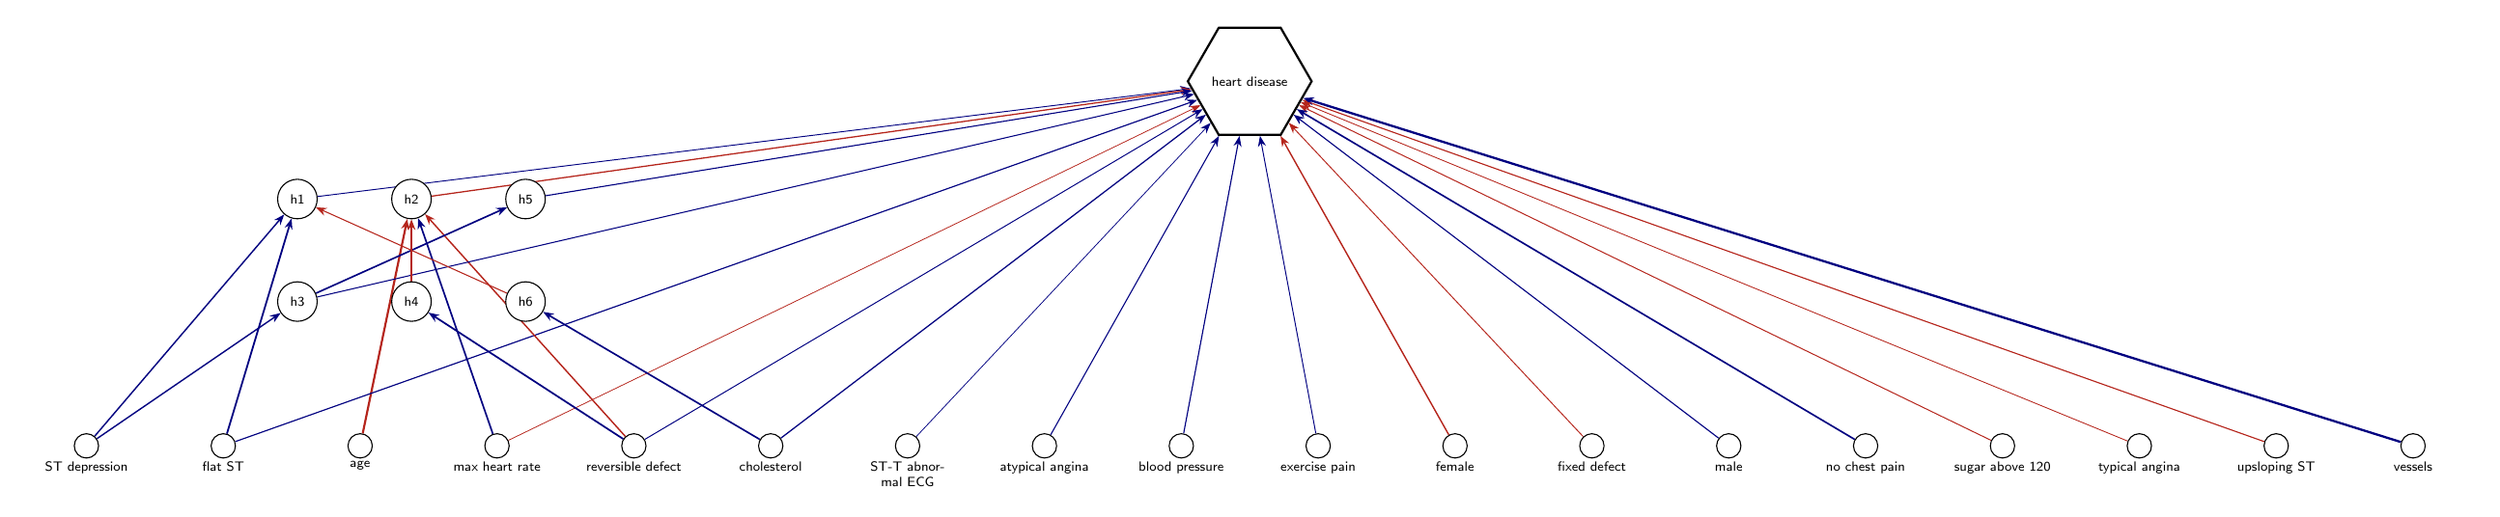
\begin{tikzpicture}[
  font=\sffamily\scriptsize, >={Stealth[length=1.4mm]},
  inp/.style={draw, circle, fill=white, minimum size=3.2mm, inner sep=0pt},
  hid/.style={draw, circle, fill=white, minimum size=5.2mm, inner sep=0.5pt, font=\sffamily\tiny},
  exitbox/.style={draw, thick, rectangle, fill=white, align=center, text width=17mm, minimum height=5mm, inner sep=1.5pt, font=\sffamily\tiny},
  sumbox/.style={draw, thick, dashed, rectangle, fill=white, align=center, text width=17mm, minimum height=5mm, inner sep=1.5pt, font=\sffamily\tiny},
  outp/.style={draw, thick, regular polygon, regular polygon sides=6, fill=white, minimum size=10mm, inner sep=0pt, font=\sffamily\tiny, align=center},
  stub/.style={draw, dashed, rounded corners=2pt, fill=white, align=center, inner sep=2pt, font=\sffamily\tiny, text width=15mm},
  inlab/.style={font=\sffamily\tiny, align=center, text width=15mm, inner sep=1pt, fill=white, fill opacity=0.8, text opacity=1},
  wpos/.style={draw=NavyBlue}, wneg/.style={draw=BrickRed}, wagg/.style={draw=black!45, line width=1.2pt},
  wmix/.style={draw=Plum},
]
\node[inp] (ninxxage) at (3.6,0.0) {};
\path (ninxxage.south) node[inlab, anchor=north] (labninxxage) {age};
\node[inp] (ninxxfbsx1) at (25.2,0.0) {};
\path (ninxxfbsx1.south) node[inlab, anchor=north] (labninxxfbsx1) {sugar above 120};
\node[inp] (ninxxrestecgx1) at (10.8,0.0) {};
\path (ninxxrestecgx1.south) node[inlab, anchor=north] (labninxxrestecgx1) {ST-T abnormal ECG};
\node[inp] (ninxxthalach) at (5.4,0.0) {};
\path (ninxxthalach.south) node[inlab, anchor=north] (labninxxthalach) {max heart rate};
\node[inp] (ninxxexangx1) at (16.2,0.0) {};
\path (ninxxexangx1.south) node[inlab, anchor=north] (labninxxexangx1) {exercise pain};
\node[inp] (ninxxoldpeak) at (0.0,0.0) {};
\path (ninxxoldpeak.south) node[inlab, anchor=north] (labninxxoldpeak) {ST depression};
\node[inp] (ninxxslopex1) at (28.8,0.0) {};
\path (ninxxslopex1.south) node[inlab, anchor=north] (labninxxslopex1) {upsloping ST};
\node[inp] (ninxxsexx0) at (18.0,0.0) {};
\path (ninxxsexx0.south) node[inlab, anchor=north] (labninxxsexx0) {female};
\node[inp] (ninxxslopex2) at (1.8,0.0) {};
\path (ninxxslopex2.south) node[inlab, anchor=north] (labninxxslopex2) {flat ST};
\node[inp] (ninxxca) at (30.6,0.0) {};
\path (ninxxca.south) node[inlab, anchor=north] (labninxxca) {vessels};
\node[inp] (ninxxthalx6) at (19.8,0.0) {};
\path (ninxxthalx6.south) node[inlab, anchor=north] (labninxxthalx6) {fixed defect};
\node[inp] (ninxxthalx7) at (7.2,0.0) {};
\path (ninxxthalx7.south) node[inlab, anchor=north] (labninxxthalx7) {reversible defect};
\node[inp] (ninxxsexx1) at (21.6,0.0) {};
\path (ninxxsexx1.south) node[inlab, anchor=north] (labninxxsexx1) {male};
\node[inp] (ninxxcpx1) at (27.0,0.0) {};
\path (ninxxcpx1.south) node[inlab, anchor=north] (labninxxcpx1) {typical angina};
\node[inp] (ninxxcpx2) at (12.6,0.0) {};
\path (ninxxcpx2.south) node[inlab, anchor=north] (labninxxcpx2) {atypical angina};
\node[inp] (ninxxcpx4) at (23.4,0.0) {};
\path (ninxxcpx4.south) node[inlab, anchor=north] (labninxxcpx4) {no chest pain};
\node[inp] (ninxxtrestbps) at (14.4,0.0) {};
\path (ninxxtrestbps.south) node[inlab, anchor=north] (labninxxtrestbps) {blood pressure};
\node[inp] (ninxxchol) at (9.0,0.0) {};
\path (ninxxchol.south) node[inlab, anchor=north] (labninxxchol) {cholesterol};
\node[outp] (n0) at (15.3,4.8) {heart disease};
\node[hid] (n1476) at (2.775,3.25) {h1};
\node[hid] (n1718) at (4.275,3.25) {h2};
\node[hid] (n1946) at (2.775,1.9) {h3};
\node[hid] (n3195) at (4.275,1.9) {h4};
\node[hid] (n3284) at (5.775,3.25) {h5};
\node[hid] (n3464) at (5.775,1.9) {h6};
\begin{scope}[on background layer]
\draw[->, wneg, line width=0.78pt] (ninxxage) -- (n1718);
\draw[->, wneg, line width=0.36pt] (ninxxfbsx1) -- (n0);
\draw[->, wpos, line width=0.27pt] (ninxxrestecgx1) -- (n0);
\draw[->, wneg, line width=0.28pt] (ninxxthalach) -- (n0);
\draw[->, wpos, line width=0.61pt] (ninxxthalach) -- (n1718);
\draw[->, wpos, line width=0.35pt] (ninxxexangx1) -- (n0);
\draw[->, wpos, line width=0.52pt] (ninxxoldpeak) -- (n1476);
\draw[->, wpos, line width=0.51pt] (ninxxoldpeak) -- (n1946);
\draw[->, wneg, line width=0.41pt] (ninxxslopex1) -- (n0);
\draw[->, wneg, line width=0.51pt] (ninxxsexx0) -- (n0);
\draw[->, wpos, line width=0.42pt] (ninxxslopex2) -- (n0);
\draw[->, wpos, line width=0.65pt] (ninxxslopex2) -- (n1476);
\draw[->, wpos, line width=0.83pt] (ninxxca) -- (n0);
\draw[->, wneg, line width=0.35pt] (ninxxthalx6) -- (n0);
\draw[->, wpos, line width=0.35pt] (ninxxthalx7) -- (n0);
\draw[->, wneg, line width=0.52pt] (ninxxthalx7) -- (n1718);
\draw[->, wpos, line width=0.63pt] (ninxxthalx7) -- (n3195);
\draw[->, wpos, line width=0.41pt] (ninxxsexx1) -- (n0);
\draw[->, wneg, line width=0.31pt] (ninxxcpx1) -- (n0);
\draw[->, wpos, line width=0.39pt] (ninxxcpx2) -- (n0);
\draw[->, wpos, line width=0.60pt] (ninxxcpx4) -- (n0);
\draw[->, wpos, line width=0.41pt] (ninxxtrestbps) -- (n0);
\draw[->, wpos, line width=0.46pt] (ninxxchol) -- (n0);
\draw[->, wpos, line width=0.60pt] (ninxxchol) -- (n3464);
\draw[->, wpos, line width=0.34pt] (n1476) -- (n0);
\draw[->, wneg, line width=0.46pt] (n1718) -- (n0);
\draw[->, wpos, line width=0.38pt] (n1946) -- (n0);
\draw[->, wpos, line width=0.60pt] (n1946) -- (n3284);
\draw[->, wneg, line width=0.51pt] (n3195) -- (n1718);
\draw[->, wpos, line width=0.40pt] (n3284) -- (n0);
\draw[->, wneg, line width=0.38pt] (n3464) -- (n1476);
\end{scope}
\end{tikzpicture}}%
\caption{The network as trained, before any explanation, in full. Blue: positive weight (raises the score); red: negative weight (lowers it); thicker: larger weight. Orange outline and up arrow: raises the final prediction; teal and down arrow: lowers it; grey and double arrow: depends. Not used (no connection): non-anginal pain, sugar 120 or less, normal ECG, LVH on ECG, no exercise pain, downsloping ST, normal thallium, thallium code 4.}
\label{fig:hearts2c1:raw}
\end{figure}
\end{landscape}
\end{drafted}
\clearpage
\end{document}
